% adopt PLoS genetics environment settings
\documentclass[10pt,letterpaper]{article}

% Load to combine multiple standalone tex files into Supplemental Material
\usepackage{standalone}

% Template for PLoS
% Version 3.2 March 2016

% General commands for the entire paper
%
% Use Unicode characters when possible
\usepackage[utf8x]{inputenc}
% amsmath package, useful for mathematical formulas
\usepackage{amsmath}
%\usepackage{natbib}
% amssymb package, useful for mathematical symbols
\usepackage{amssymb}
\usepackage{booktabs}
\usepackage{xspace}
\usepackage{hyperref}
% graphicx package, useful for including eps and pdf graphics
% include graphics with the command \includegraphics
\usepackage{graphicx}

% Use adjustwidth environment to exceed column width (see example table in text)
\usepackage{changepage}

% textcomp package and marvosym package for additional characters
\usepackage{textcomp,marvosym}

% fixltx2e package for \textsubscript
\usepackage{fixltx2e}

% cite package, to clean up citations in the main text. Do not remove.
\usepackage{cite}
\usepackage{caption}
\usepackage{subcaption}
\usepackage{rotating}

\usepackage{color}

% Use doublespacing - comment out for single spacing
%\usepackage{setspace}
%\doublespacing

% Text layout
\topmargin 0.0cm
\oddsidemargin 0.5cm
\evensidemargin 0.5cm
\textwidth 16cm
\textheight 21cm

\setlength{\parskip}{1em}

% Bold the 'Figure #' in the caption and separate it with a period
% Captions will be left justified
\usepackage[labelfont=bf,labelsep=period,justification=raggedright]{caption}

% Use the PLoS provided bibtex style
\bibliographystyle{/Users/stephens/Dropbox/Documents/stylefiles/plos2009}

% Remove brackets from numbering in List of References
\makeatletter
\renewcommand{\@biblabel}[1]{\quad#1.}
\makeatother

% Use nameref to cite supporting information files (see Supporting Information section for more info)
\usepackage{nameref,hyperref}

% line numbers
\usepackage[right]{lineno}

% ligatures disabled
\usepackage{microtype}
\DisableLigatures[f]{encoding = *, family = * }

% Leave date blank
\date{}

\pagestyle{myheadings}
%% ** EDIT HERE **
\usepackage{enumerate}
\usepackage{multirow}
\usepackage{url}
\usepackage{xr} %for cross-referencing
%% ** EDIT HERE **
%% PLEASE INCLUDE ALL MACROS BELOW
\newtheorem{algorithm}{Algorithm}
\newtheorem{proposition}{Proposition}
\newtheorem{restateproposition}{Proposition}
\newtheorem{lemma}{Lemma}
\newtheorem{corollary}{Corollary}
\newtheorem{result}{Result}
\newtheorem{note}{Note}
\newtheorem{definition}{Definition}

\def\KL{\text{KL}}


% Text layout
\raggedright
\setlength{\parindent}{0.5cm}
\textwidth 5.25in
\textheight 8.75in

% Bold the 'Figure #' in the caption and separate it from the title/caption with a period
% Captions will be left justified
\usepackage[aboveskip=1pt,labelfont=bf,labelsep=period,justification=raggedright,singlelinecheck=off]{caption}
\renewcommand{\figurename}{Fig}

%------ bibliography
% Use the PLoS provided BiBTeX style
\bibliographystyle{plos2015}
% Remove brackets from numbering in List of References
\makeatletter
\renewcommand{\@biblabel}[1]{\quad#1.}
\makeatother


% Header and Footer with logo
\usepackage{lastpage,fancyhdr,graphicx}
\usepackage{epstopdf}
\pagestyle{myheadings}
\pagestyle{fancy}
\fancyhf{}
\setlength{\headheight}{27.023pt}
\lhead{\includegraphics[width=2.0in]{PLOS-submission.eps}}
\rfoot{\thepage/\pageref{LastPage}}
\renewcommand{\footrule}{\hrule height 2pt \vspace{2mm}}
\fancyheadoffset[L]{2.25in}
\fancyfootoffset[L]{2.25in}
\lfoot{\sf PLOS}

%% Include all macros below

\newcommand{\lorem}{{\bf LOREM}}
\newcommand{\ipsum}{{\bf IPSUM}}

%% END MACROS SECTION

%% Author's settings
\def\KL{\text{KL}}


% Text layout specific to Supplemental Materials
\topmargin 0.0cm
\oddsidemargin 0.5cm
\evensidemargin 0.5cm
\textwidth 16cm
\textheight 21cm

\setlength{\parskip}{1em}

\begin{document}

\section{Supplementary figures}
% adopt PLoS genetics environment settings
\documentclass[10pt,letterpaper]{article}
\usepackage[top=0.85in,left=2.75in,footskip=0.75in]{geometry}

% Template for PLoS
% Version 3.2 March 2016

% General commands for the entire paper
%
% Use Unicode characters when possible
\usepackage[utf8x]{inputenc}
% amsmath package, useful for mathematical formulas
\usepackage{amsmath}
%\usepackage{natbib}
% amssymb package, useful for mathematical symbols
\usepackage{amssymb}
\usepackage{booktabs}
\usepackage{xspace}
\usepackage{hyperref}
% graphicx package, useful for including eps and pdf graphics
% include graphics with the command \includegraphics
\usepackage{graphicx}

% Use adjustwidth environment to exceed column width (see example table in text)
\usepackage{changepage}

% textcomp package and marvosym package for additional characters
\usepackage{textcomp,marvosym}

% fixltx2e package for \textsubscript
\usepackage{fixltx2e}

% cite package, to clean up citations in the main text. Do not remove.
\usepackage{cite}
\usepackage{caption}
\usepackage{subcaption}
\usepackage{rotating}

\usepackage{color}

% Use doublespacing - comment out for single spacing
%\usepackage{setspace}
%\doublespacing

% Text layout
\topmargin 0.0cm
\oddsidemargin 0.5cm
\evensidemargin 0.5cm
\textwidth 16cm
\textheight 21cm

\setlength{\parskip}{1em}

% Bold the 'Figure #' in the caption and separate it with a period
% Captions will be left justified
\usepackage[labelfont=bf,labelsep=period,justification=raggedright]{caption}

% Use the PLoS provided bibtex style
\bibliographystyle{/Users/stephens/Dropbox/Documents/stylefiles/plos2009}

% Remove brackets from numbering in List of References
\makeatletter
\renewcommand{\@biblabel}[1]{\quad#1.}
\makeatother

% Use nameref to cite supporting information files (see Supporting Information section for more info)
\usepackage{nameref,hyperref}

% line numbers
\usepackage[right]{lineno}

% ligatures disabled
\usepackage{microtype}
\DisableLigatures[f]{encoding = *, family = * }

% Leave date blank
\date{}

\pagestyle{myheadings}
%% ** EDIT HERE **
\usepackage{enumerate}
\usepackage{multirow}
\usepackage{url}
\usepackage{xr} %for cross-referencing
%% ** EDIT HERE **
%% PLEASE INCLUDE ALL MACROS BELOW
\newtheorem{algorithm}{Algorithm}
\newtheorem{proposition}{Proposition}
\newtheorem{restateproposition}{Proposition}
\newtheorem{lemma}{Lemma}
\newtheorem{corollary}{Corollary}
\newtheorem{result}{Result}
\newtheorem{note}{Note}
\newtheorem{definition}{Definition}

\def\KL{\text{KL}}


% Text layout
\raggedright
\setlength{\parindent}{0.5cm}
\textwidth 5.25in
\textheight 8.75in

% Bold the 'Figure #' in the caption and separate it from the title/caption with a period
% Captions will be left justified
\usepackage[aboveskip=1pt,labelfont=bf,labelsep=period,justification=raggedright,singlelinecheck=off]{caption}
\renewcommand{\figurename}{Fig}

%------ bibliography
% Use the PLoS provided BiBTeX style
\bibliographystyle{plos2015}
% Remove brackets from numbering in List of References
\makeatletter
\renewcommand{\@biblabel}[1]{\quad#1.}
\makeatother


% Header and Footer with logo
\usepackage{lastpage,fancyhdr,graphicx}
\usepackage{epstopdf}
\pagestyle{myheadings}
\pagestyle{fancy}
\fancyhf{}
\setlength{\headheight}{27.023pt}
\lhead{\includegraphics[width=2.0in]{PLOS-submission.eps}}
\rfoot{\thepage/\pageref{LastPage}}
\renewcommand{\footrule}{\hrule height 2pt \vspace{2mm}}
\fancyheadoffset[L]{2.25in}
\fancyfootoffset[L]{2.25in}
\lfoot{\sf PLOS}

%% Include all macros below

\newcommand{\lorem}{{\bf LOREM}}
\newcommand{\ipsum}{{\bf IPSUM}}

%% END MACROS SECTION

%% Author's settings
\def\KL{\text{KL}}


% Text layout specific to Supplemental Materials
\topmargin 0.0cm
\oddsidemargin 0.5cm
\evensidemargin 0.5cm
\textwidth 16cm
\textheight 21cm

\setlength{\parskip}{1em}

\begin{document}

\paragraph{S1 Fig.}
\label{figS1}
{\bf Structure plot of GTEx V6 all tissue samples for (a) $K=5$, (b) $K=10$, (c) $K=15$, (d) $K=20$.} Some tissues form a separate cluster from the rest of the tissues from $K=5$ onwards (for example: Whole Blood, Skin), whereas some tissues only form a distinctive subgroup only at $K=20$ (for example: Arteries).
\begin{figure}[ht]
\centering
\includegraphics[height=7.5in, width=6.5in]{../../plots/gtex-figures/gtex-multiple-ks-04-30-2016}
\end{figure}

\end{document}

\clearpage
% adopt PLoS genetics environment settings
\documentclass[10pt,letterpaper]{article}
\usepackage[top=0.85in,left=2.75in,footskip=0.75in]{geometry}

% Template for PLoS
% Version 3.2 March 2016

% General commands for the entire paper
%
% Use Unicode characters when possible
\usepackage[utf8x]{inputenc}
% amsmath package, useful for mathematical formulas
\usepackage{amsmath}
%\usepackage{natbib}
% amssymb package, useful for mathematical symbols
\usepackage{amssymb}
\usepackage{booktabs}
\usepackage{xspace}
\usepackage{hyperref}
% graphicx package, useful for including eps and pdf graphics
% include graphics with the command \includegraphics
\usepackage{graphicx}

% Use adjustwidth environment to exceed column width (see example table in text)
\usepackage{changepage}

% textcomp package and marvosym package for additional characters
\usepackage{textcomp,marvosym}

% fixltx2e package for \textsubscript
\usepackage{fixltx2e}

% cite package, to clean up citations in the main text. Do not remove.
\usepackage{cite}
\usepackage{caption}
\usepackage{subcaption}
\usepackage{rotating}

\usepackage{color}

% Use doublespacing - comment out for single spacing
%\usepackage{setspace}
%\doublespacing

% Text layout
\topmargin 0.0cm
\oddsidemargin 0.5cm
\evensidemargin 0.5cm
\textwidth 16cm
\textheight 21cm

\setlength{\parskip}{1em}

% Bold the 'Figure #' in the caption and separate it with a period
% Captions will be left justified
\usepackage[labelfont=bf,labelsep=period,justification=raggedright]{caption}

% Use the PLoS provided bibtex style
\bibliographystyle{/Users/stephens/Dropbox/Documents/stylefiles/plos2009}

% Remove brackets from numbering in List of References
\makeatletter
\renewcommand{\@biblabel}[1]{\quad#1.}
\makeatother

% Use nameref to cite supporting information files (see Supporting Information section for more info)
\usepackage{nameref,hyperref}

% line numbers
\usepackage[right]{lineno}

% ligatures disabled
\usepackage{microtype}
\DisableLigatures[f]{encoding = *, family = * }

% Leave date blank
\date{}

\pagestyle{myheadings}
%% ** EDIT HERE **
\usepackage{enumerate}
\usepackage{multirow}
\usepackage{url}
\usepackage{xr} %for cross-referencing
%% ** EDIT HERE **
%% PLEASE INCLUDE ALL MACROS BELOW
\newtheorem{algorithm}{Algorithm}
\newtheorem{proposition}{Proposition}
\newtheorem{restateproposition}{Proposition}
\newtheorem{lemma}{Lemma}
\newtheorem{corollary}{Corollary}
\newtheorem{result}{Result}
\newtheorem{note}{Note}
\newtheorem{definition}{Definition}

\def\KL{\text{KL}}


% Text layout
\raggedright
\setlength{\parindent}{0.5cm}
\textwidth 5.25in
\textheight 8.75in

% Bold the 'Figure #' in the caption and separate it from the title/caption with a period
% Captions will be left justified
\usepackage[aboveskip=1pt,labelfont=bf,labelsep=period,justification=raggedright,singlelinecheck=off]{caption}
\renewcommand{\figurename}{Fig}

%------ bibliography
% Use the PLoS provided BiBTeX style
\bibliographystyle{plos2015}
% Remove brackets from numbering in List of References
\makeatletter
\renewcommand{\@biblabel}[1]{\quad#1.}
\makeatother


% Header and Footer with logo
\usepackage{lastpage,fancyhdr,graphicx}
\usepackage{epstopdf}
\pagestyle{myheadings}
\pagestyle{fancy}
\fancyhf{}
\setlength{\headheight}{27.023pt}
\lhead{\includegraphics[width=2.0in]{PLOS-submission.eps}}
\rfoot{\thepage/\pageref{LastPage}}
\renewcommand{\footrule}{\hrule height 2pt \vspace{2mm}}
\fancyheadoffset[L]{2.25in}
\fancyfootoffset[L]{2.25in}
\lfoot{\sf PLOS}

%% Include all macros below

\newcommand{\lorem}{{\bf LOREM}}
\newcommand{\ipsum}{{\bf IPSUM}}

%% END MACROS SECTION

%% Author's settings
\def\KL{\text{KL}}


% Text layout specific to Supplemental Materials
\topmargin 0.0cm
\oddsidemargin 0.5cm
\evensidemargin 0.5cm
\textwidth 16cm
\textheight 21cm

\setlength{\parskip}{1em}

\begin{document}

\paragraph{S2 Fig.}
\label{figS2}
{\bf Structure plot of GTEx V6 tissue samples for $K=20$ in two runs under different thinning parameter settings.} (A) $p_{thin}=0.01$ and (B) $p_{thin}=0.0001$.} The structural patterns in these two plots closely resemble the structural patterns in Fig~1(a), though there are a few differences from the unthinned version.
\begin{figure}[ht]
\centering
\includegraphics[height=7.5in, width=6.5in]{../../plots/gtex-figures/gtex_thinned_04_25_2016.pdf}
\end{figure}
\clearpage

\end{document}

\clearpage
% adopt PLoS genetics environment settings
\documentclass[10pt,letterpaper]{article}
\usepackage[top=0.85in,left=2.75in,footskip=0.75in]{geometry}

% Template for PLoS
% Version 3.2 March 2016

% General commands for the entire paper
%
% Use Unicode characters when possible
\usepackage[utf8x]{inputenc}
% amsmath package, useful for mathematical formulas
\usepackage{amsmath}
%\usepackage{natbib}
% amssymb package, useful for mathematical symbols
\usepackage{amssymb}
\usepackage{booktabs}
\usepackage{xspace}
\usepackage{hyperref}
% graphicx package, useful for including eps and pdf graphics
% include graphics with the command \includegraphics
\usepackage{graphicx}

% Use adjustwidth environment to exceed column width (see example table in text)
\usepackage{changepage}

% textcomp package and marvosym package for additional characters
\usepackage{textcomp,marvosym}

% fixltx2e package for \textsubscript
\usepackage{fixltx2e}

% cite package, to clean up citations in the main text. Do not remove.
\usepackage{cite}
\usepackage{caption}
\usepackage{subcaption}
\usepackage{rotating}

\usepackage{color}

% Use doublespacing - comment out for single spacing
%\usepackage{setspace}
%\doublespacing

% Text layout
\topmargin 0.0cm
\oddsidemargin 0.5cm
\evensidemargin 0.5cm
\textwidth 16cm
\textheight 21cm

\setlength{\parskip}{1em}

% Bold the 'Figure #' in the caption and separate it with a period
% Captions will be left justified
\usepackage[labelfont=bf,labelsep=period,justification=raggedright]{caption}

% Use the PLoS provided bibtex style
\bibliographystyle{/Users/stephens/Dropbox/Documents/stylefiles/plos2009}

% Remove brackets from numbering in List of References
\makeatletter
\renewcommand{\@biblabel}[1]{\quad#1.}
\makeatother

% Use nameref to cite supporting information files (see Supporting Information section for more info)
\usepackage{nameref,hyperref}

% line numbers
\usepackage[right]{lineno}

% ligatures disabled
\usepackage{microtype}
\DisableLigatures[f]{encoding = *, family = * }

% Leave date blank
\date{}

\pagestyle{myheadings}
%% ** EDIT HERE **
\usepackage{enumerate}
\usepackage{multirow}
\usepackage{url}
\usepackage{xr} %for cross-referencing
%% ** EDIT HERE **
%% PLEASE INCLUDE ALL MACROS BELOW
\newtheorem{algorithm}{Algorithm}
\newtheorem{proposition}{Proposition}
\newtheorem{restateproposition}{Proposition}
\newtheorem{lemma}{Lemma}
\newtheorem{corollary}{Corollary}
\newtheorem{result}{Result}
\newtheorem{note}{Note}
\newtheorem{definition}{Definition}

\def\KL{\text{KL}}


% Text layout
\raggedright
\setlength{\parindent}{0.5cm}
\textwidth 5.25in
\textheight 8.75in

% Bold the 'Figure #' in the caption and separate it from the title/caption with a period
% Captions will be left justified
\usepackage[aboveskip=1pt,labelfont=bf,labelsep=period,justification=raggedright,singlelinecheck=off]{caption}
\renewcommand{\figurename}{Fig}

%------ bibliography
% Use the PLoS provided BiBTeX style
\bibliographystyle{plos2015}
% Remove brackets from numbering in List of References
\makeatletter
\renewcommand{\@biblabel}[1]{\quad#1.}
\makeatother


% Header and Footer with logo
\usepackage{lastpage,fancyhdr,graphicx}
\usepackage{epstopdf}
\pagestyle{myheadings}
\pagestyle{fancy}
\fancyhf{}
\setlength{\headheight}{27.023pt}
\lhead{\includegraphics[width=2.0in]{PLOS-submission.eps}}
\rfoot{\thepage/\pageref{LastPage}}
\renewcommand{\footrule}{\hrule height 2pt \vspace{2mm}}
\fancyheadoffset[L]{2.25in}
\fancyfootoffset[L]{2.25in}
\lfoot{\sf PLOS}

%% Include all macros below

\newcommand{\lorem}{{\bf LOREM}}
\newcommand{\ipsum}{{\bf IPSUM}}

%% END MACROS SECTION

%% Author's settings
\def\KL{\text{KL}}


\begin{document}

\paragraph*{S3 Fig.}
\label{figS3}
{\bf A comparison of ``accuracy" of hierarchical vs. model-based clustering on thinned GTEx data, with thinning parameter $p_{thin}=0.01$ and $p_{thin}=0.0001$.}  For each pair of tissues from the GTEx data we assessed whether or not each clustering method (with $K=2$ clusters) separated the samples according to their actual tissue of origin, with successful separation indicated by a filled square. Thinning deteriorates accuracy compared with the unthinned data (Fig~2), but even then the model-based method remains more successful than the hierarchical clustering in separating the samples by tissue or origin.
 \begin{figure*}[ht]
    \centering
     \begin{subfigure}[t]{0.5\textwidth}
        \centering
        \includegraphics[height=2.5in]{../../plots/rsz_1hierarchy_F_thin_0_01.png}
        \caption{hierarchy thin 0.01}
    \end{subfigure}%
    ~
    \begin{subfigure}[t]{0.5\textwidth}
        \centering
        \includegraphics[height=2.5in]{../../plots/rsz_1hierarchy_F_thin_0_01.png}
        \caption{GoM thin 0.01}
    \end{subfigure}\\

     \begin{subfigure}[t]{0.5\textwidth}
        \centering
        \includegraphics[height=2.5in]{../../plots/rsz_1hierarchy_F_thin_0_0001.png}
        \caption{hierarchy 0.0001}
    \end{subfigure}%
    ~
    \begin{subfigure}[t]{0.5\textwidth}
        \centering
        \includegraphics[height=2.5in]{../../plots/rsz_1admixture_F_thin_0_0001.png}
        \caption{GoM thin 0.0001}
    \end{subfigure}\\
\end{figure*}

\end{document}

\clearpage
% adopt PLoS genetics environment settings
\documentclass[10pt,letterpaper]{article}
\usepackage[top=0.85in,left=2.75in,footskip=0.75in]{geometry}

% Template for PLoS
% Version 3.2 March 2016

% General commands for the entire paper
%
% Use Unicode characters when possible
\usepackage[utf8x]{inputenc}
% amsmath package, useful for mathematical formulas
\usepackage{amsmath}
%\usepackage{natbib}
% amssymb package, useful for mathematical symbols
\usepackage{amssymb}
\usepackage{booktabs}
\usepackage{xspace}
\usepackage{hyperref}
% graphicx package, useful for including eps and pdf graphics
% include graphics with the command \includegraphics
\usepackage{graphicx}

% Use adjustwidth environment to exceed column width (see example table in text)
\usepackage{changepage}

% textcomp package and marvosym package for additional characters
\usepackage{textcomp,marvosym}

% fixltx2e package for \textsubscript
\usepackage{fixltx2e}

% cite package, to clean up citations in the main text. Do not remove.
\usepackage{cite}
\usepackage{caption}
\usepackage{subcaption}
\usepackage{rotating}

\usepackage{color}

% Use doublespacing - comment out for single spacing
%\usepackage{setspace}
%\doublespacing

% Text layout
\topmargin 0.0cm
\oddsidemargin 0.5cm
\evensidemargin 0.5cm
\textwidth 16cm
\textheight 21cm

\setlength{\parskip}{1em}

% Bold the 'Figure #' in the caption and separate it with a period
% Captions will be left justified
\usepackage[labelfont=bf,labelsep=period,justification=raggedright]{caption}

% Use the PLoS provided bibtex style
\bibliographystyle{/Users/stephens/Dropbox/Documents/stylefiles/plos2009}

% Remove brackets from numbering in List of References
\makeatletter
\renewcommand{\@biblabel}[1]{\quad#1.}
\makeatother

% Use nameref to cite supporting information files (see Supporting Information section for more info)
\usepackage{nameref,hyperref}

% line numbers
\usepackage[right]{lineno}

% ligatures disabled
\usepackage{microtype}
\DisableLigatures[f]{encoding = *, family = * }

% Leave date blank
\date{}

\pagestyle{myheadings}
%% ** EDIT HERE **
\usepackage{enumerate}
\usepackage{multirow}
\usepackage{url}
\usepackage{xr} %for cross-referencing
%% ** EDIT HERE **
%% PLEASE INCLUDE ALL MACROS BELOW
\newtheorem{algorithm}{Algorithm}
\newtheorem{proposition}{Proposition}
\newtheorem{restateproposition}{Proposition}
\newtheorem{lemma}{Lemma}
\newtheorem{corollary}{Corollary}
\newtheorem{result}{Result}
\newtheorem{note}{Note}
\newtheorem{definition}{Definition}

\def\KL{\text{KL}}


% Text layout
\raggedright
\setlength{\parindent}{0.5cm}
\textwidth 5.25in
\textheight 8.75in

% Bold the 'Figure #' in the caption and separate it from the title/caption with a period
% Captions will be left justified
\usepackage[aboveskip=1pt,labelfont=bf,labelsep=period,justification=raggedright,singlelinecheck=off]{caption}
\renewcommand{\figurename}{Fig}

%------ bibliography
% Use the PLoS provided BiBTeX style
\bibliographystyle{plos2015}
% Remove brackets from numbering in List of References
\makeatletter
\renewcommand{\@biblabel}[1]{\quad#1.}
\makeatother


% Header and Footer with logo
\usepackage{lastpage,fancyhdr,graphicx}
\usepackage{epstopdf}
\pagestyle{myheadings}
\pagestyle{fancy}
\fancyhf{}
\setlength{\headheight}{27.023pt}
\lhead{\includegraphics[width=2.0in]{PLOS-submission.eps}}
\rfoot{\thepage/\pageref{LastPage}}
\renewcommand{\footrule}{\hrule height 2pt \vspace{2mm}}
\fancyheadoffset[L]{2.25in}
\fancyfootoffset[L]{2.25in}
\lfoot{\sf PLOS}

%% Include all macros below

\newcommand{\lorem}{{\bf LOREM}}
\newcommand{\ipsum}{{\bf IPSUM}}

%% END MACROS SECTION

%% Author's settings
\def\KL{\text{KL}}


% Text layout specific to Supplemental Materials
\topmargin 0.0cm
\oddsidemargin 0.5cm
\evensidemargin 0.5cm
\textwidth 16cm
\textheight 21cm

\setlength{\parskip}{1em}

\begin{document}

\paragraph*{S4 Fig.}

\label{figS4}
{\bf GTEx data visualization of all tissue samples using (a) principle component analysis and (b) t-SNE
(c) Multidimensional scaling.}
Samples of matching tissue types are indicated by points of matching color.
\begin{figure}[ht]
\centering
\includegraphics[height=6in, width=5in]{../../src/figure/gtex-other-methods.Rmd/gtex-with-legend.png}
\end{figure}

\end{document}

\clearpage
% adopt PLoS genetics environment settings
\documentclass[10pt,letterpaper]{article}
\usepackage[top=0.85in,left=2.75in,footskip=0.75in]{geometry}

% Template for PLoS
% Version 3.2 March 2016

% General commands for the entire paper
%
% Use Unicode characters when possible
\usepackage[utf8x]{inputenc}
% amsmath package, useful for mathematical formulas
\usepackage{amsmath}
%\usepackage{natbib}
% amssymb package, useful for mathematical symbols
\usepackage{amssymb}
\usepackage{booktabs}
\usepackage{xspace}
\usepackage{hyperref}
% graphicx package, useful for including eps and pdf graphics
% include graphics with the command \includegraphics
\usepackage{graphicx}

% Use adjustwidth environment to exceed column width (see example table in text)
\usepackage{changepage}

% textcomp package and marvosym package for additional characters
\usepackage{textcomp,marvosym}

% fixltx2e package for \textsubscript
\usepackage{fixltx2e}

% cite package, to clean up citations in the main text. Do not remove.
\usepackage{cite}
\usepackage{caption}
\usepackage{subcaption}
\usepackage{rotating}

\usepackage{color}

% Use doublespacing - comment out for single spacing
%\usepackage{setspace}
%\doublespacing

% Text layout
\topmargin 0.0cm
\oddsidemargin 0.5cm
\evensidemargin 0.5cm
\textwidth 16cm
\textheight 21cm

\setlength{\parskip}{1em}

% Bold the 'Figure #' in the caption and separate it with a period
% Captions will be left justified
\usepackage[labelfont=bf,labelsep=period,justification=raggedright]{caption}

% Use the PLoS provided bibtex style
\bibliographystyle{/Users/stephens/Dropbox/Documents/stylefiles/plos2009}

% Remove brackets from numbering in List of References
\makeatletter
\renewcommand{\@biblabel}[1]{\quad#1.}
\makeatother

% Use nameref to cite supporting information files (see Supporting Information section for more info)
\usepackage{nameref,hyperref}

% line numbers
\usepackage[right]{lineno}

% ligatures disabled
\usepackage{microtype}
\DisableLigatures[f]{encoding = *, family = * }

% Leave date blank
\date{}

\pagestyle{myheadings}
%% ** EDIT HERE **
\usepackage{enumerate}
\usepackage{multirow}
\usepackage{url}
\usepackage{xr} %for cross-referencing
%% ** EDIT HERE **
%% PLEASE INCLUDE ALL MACROS BELOW
\newtheorem{algorithm}{Algorithm}
\newtheorem{proposition}{Proposition}
\newtheorem{restateproposition}{Proposition}
\newtheorem{lemma}{Lemma}
\newtheorem{corollary}{Corollary}
\newtheorem{result}{Result}
\newtheorem{note}{Note}
\newtheorem{definition}{Definition}

\def\KL{\text{KL}}


% Text layout
\raggedright
\setlength{\parindent}{0.5cm}
\textwidth 5.25in
\textheight 8.75in

% Bold the 'Figure #' in the caption and separate it from the title/caption with a period
% Captions will be left justified
\usepackage[aboveskip=1pt,labelfont=bf,labelsep=period,justification=raggedright,singlelinecheck=off]{caption}
\renewcommand{\figurename}{Fig}

%------ bibliography
% Use the PLoS provided BiBTeX style
\bibliographystyle{plos2015}
% Remove brackets from numbering in List of References
\makeatletter
\renewcommand{\@biblabel}[1]{\quad#1.}
\makeatother


% Header and Footer with logo
\usepackage{lastpage,fancyhdr,graphicx}
\usepackage{epstopdf}
\pagestyle{myheadings}
\pagestyle{fancy}
\fancyhf{}
\setlength{\headheight}{27.023pt}
\lhead{\includegraphics[width=2.0in]{PLOS-submission.eps}}
\rfoot{\thepage/\pageref{LastPage}}
\renewcommand{\footrule}{\hrule height 2pt \vspace{2mm}}
\fancyheadoffset[L]{2.25in}
\fancyfootoffset[L]{2.25in}
\lfoot{\sf PLOS}

%% Include all macros below

\newcommand{\lorem}{{\bf LOREM}}
\newcommand{\ipsum}{{\bf IPSUM}}

%% END MACROS SECTION

%% Author's settings
\def\KL{\text{KL}}


\begin{document}

\paragraph*{S5 Fig.}

\label{figS5}
{\bf Mouse embryo single cell sample visualization using principle component analysis and t-SNE.
\begin{figure*}[ht]
\centering
\includegraphics[height=2.5in, width=6.5in]{../../src/figure/deng-pca-vs-tsne.Rmd/deng-with-legend.jpeg}
 \caption{ Visualization of mouse early embryo samples.
            Points of matching color represent single cell samples collected at the same developmental stage.
          \textbf{(A)}: Samples plotted in PC1 versus PC2. \textbf{(B)} t-SNE 1st versus 2nd dimension.}
\end{figure*}

\end{document}

\clearpage
% adopt PLoS genetics environment settings
\documentclass[10pt,letterpaper]{article}
\usepackage[top=0.85in,left=2.75in,footskip=0.75in]{geometry}

% Template for PLoS
% Version 3.2 March 2016

% General commands for the entire paper
%
% Use Unicode characters when possible
\usepackage[utf8x]{inputenc}
% amsmath package, useful for mathematical formulas
\usepackage{amsmath}
%\usepackage{natbib}
% amssymb package, useful for mathematical symbols
\usepackage{amssymb}
\usepackage{booktabs}
\usepackage{xspace}
\usepackage{hyperref}
% graphicx package, useful for including eps and pdf graphics
% include graphics with the command \includegraphics
\usepackage{graphicx}

% Use adjustwidth environment to exceed column width (see example table in text)
\usepackage{changepage}

% textcomp package and marvosym package for additional characters
\usepackage{textcomp,marvosym}

% fixltx2e package for \textsubscript
\usepackage{fixltx2e}

% cite package, to clean up citations in the main text. Do not remove.
\usepackage{cite}
\usepackage{caption}
\usepackage{subcaption}
\usepackage{rotating}

\usepackage{color}

% Use doublespacing - comment out for single spacing
%\usepackage{setspace}
%\doublespacing

% Text layout
\topmargin 0.0cm
\oddsidemargin 0.5cm
\evensidemargin 0.5cm
\textwidth 16cm
\textheight 21cm

\setlength{\parskip}{1em}

% Bold the 'Figure #' in the caption and separate it with a period
% Captions will be left justified
\usepackage[labelfont=bf,labelsep=period,justification=raggedright]{caption}

% Use the PLoS provided bibtex style
\bibliographystyle{/Users/stephens/Dropbox/Documents/stylefiles/plos2009}

% Remove brackets from numbering in List of References
\makeatletter
\renewcommand{\@biblabel}[1]{\quad#1.}
\makeatother

% Use nameref to cite supporting information files (see Supporting Information section for more info)
\usepackage{nameref,hyperref}

% line numbers
\usepackage[right]{lineno}

% ligatures disabled
\usepackage{microtype}
\DisableLigatures[f]{encoding = *, family = * }

% Leave date blank
\date{}

\pagestyle{myheadings}
%% ** EDIT HERE **
\usepackage{enumerate}
\usepackage{multirow}
\usepackage{url}
\usepackage{xr} %for cross-referencing
%% ** EDIT HERE **
%% PLEASE INCLUDE ALL MACROS BELOW
\newtheorem{algorithm}{Algorithm}
\newtheorem{proposition}{Proposition}
\newtheorem{restateproposition}{Proposition}
\newtheorem{lemma}{Lemma}
\newtheorem{corollary}{Corollary}
\newtheorem{result}{Result}
\newtheorem{note}{Note}
\newtheorem{definition}{Definition}

\def\KL{\text{KL}}


% Text layout
\raggedright
\setlength{\parindent}{0.5cm}
\textwidth 5.25in
\textheight 8.75in

% Bold the 'Figure #' in the caption and separate it from the title/caption with a period
% Captions will be left justified
\usepackage[aboveskip=1pt,labelfont=bf,labelsep=period,justification=raggedright,singlelinecheck=off]{caption}
\renewcommand{\figurename}{Fig}

%------ bibliography
% Use the PLoS provided BiBTeX style
\bibliographystyle{plos2015}
% Remove brackets from numbering in List of References
\makeatletter
\renewcommand{\@biblabel}[1]{\quad#1.}
\makeatother


% Header and Footer with logo
\usepackage{lastpage,fancyhdr,graphicx}
\usepackage{epstopdf}
\pagestyle{myheadings}
\pagestyle{fancy}
\fancyhf{}
\setlength{\headheight}{27.023pt}
\lhead{\includegraphics[width=2.0in]{PLOS-submission.eps}}
\rfoot{\thepage/\pageref{LastPage}}
\renewcommand{\footrule}{\hrule height 2pt \vspace{2mm}}
\fancyheadoffset[L]{2.25in}
\fancyfootoffset[L]{2.25in}
\lfoot{\sf PLOS}

%% Include all macros below

\newcommand{\lorem}{{\bf LOREM}}
\newcommand{\ipsum}{{\bf IPSUM}}

%% END MACROS SECTION

%% Author's settings
\def\KL{\text{KL}}


% Text layout specific to Supplemental Materials
\topmargin 0.0cm
\oddsidemargin 0.5cm
\evensidemargin 0.5cm
\textwidth 16cm
\textheight 21cm

\setlength{\parskip}{1em}

\begin{document}

\paragraph*{S6 Fig.}

\label{figS6}
{\bf Visualization of loadings from Sparse Factor Analysis on GTEx data.} Stacked bar chart visualization of loadings Sparse Factor Analysis (SFA) on $8555$ tissue samples
across the 53 tissue types in GTEx V6 data. \textbf{(left)}: when the loadings are sparse. \textbf{(right)} when the factors are sparse.
\begin{figure}[ht]
\centering
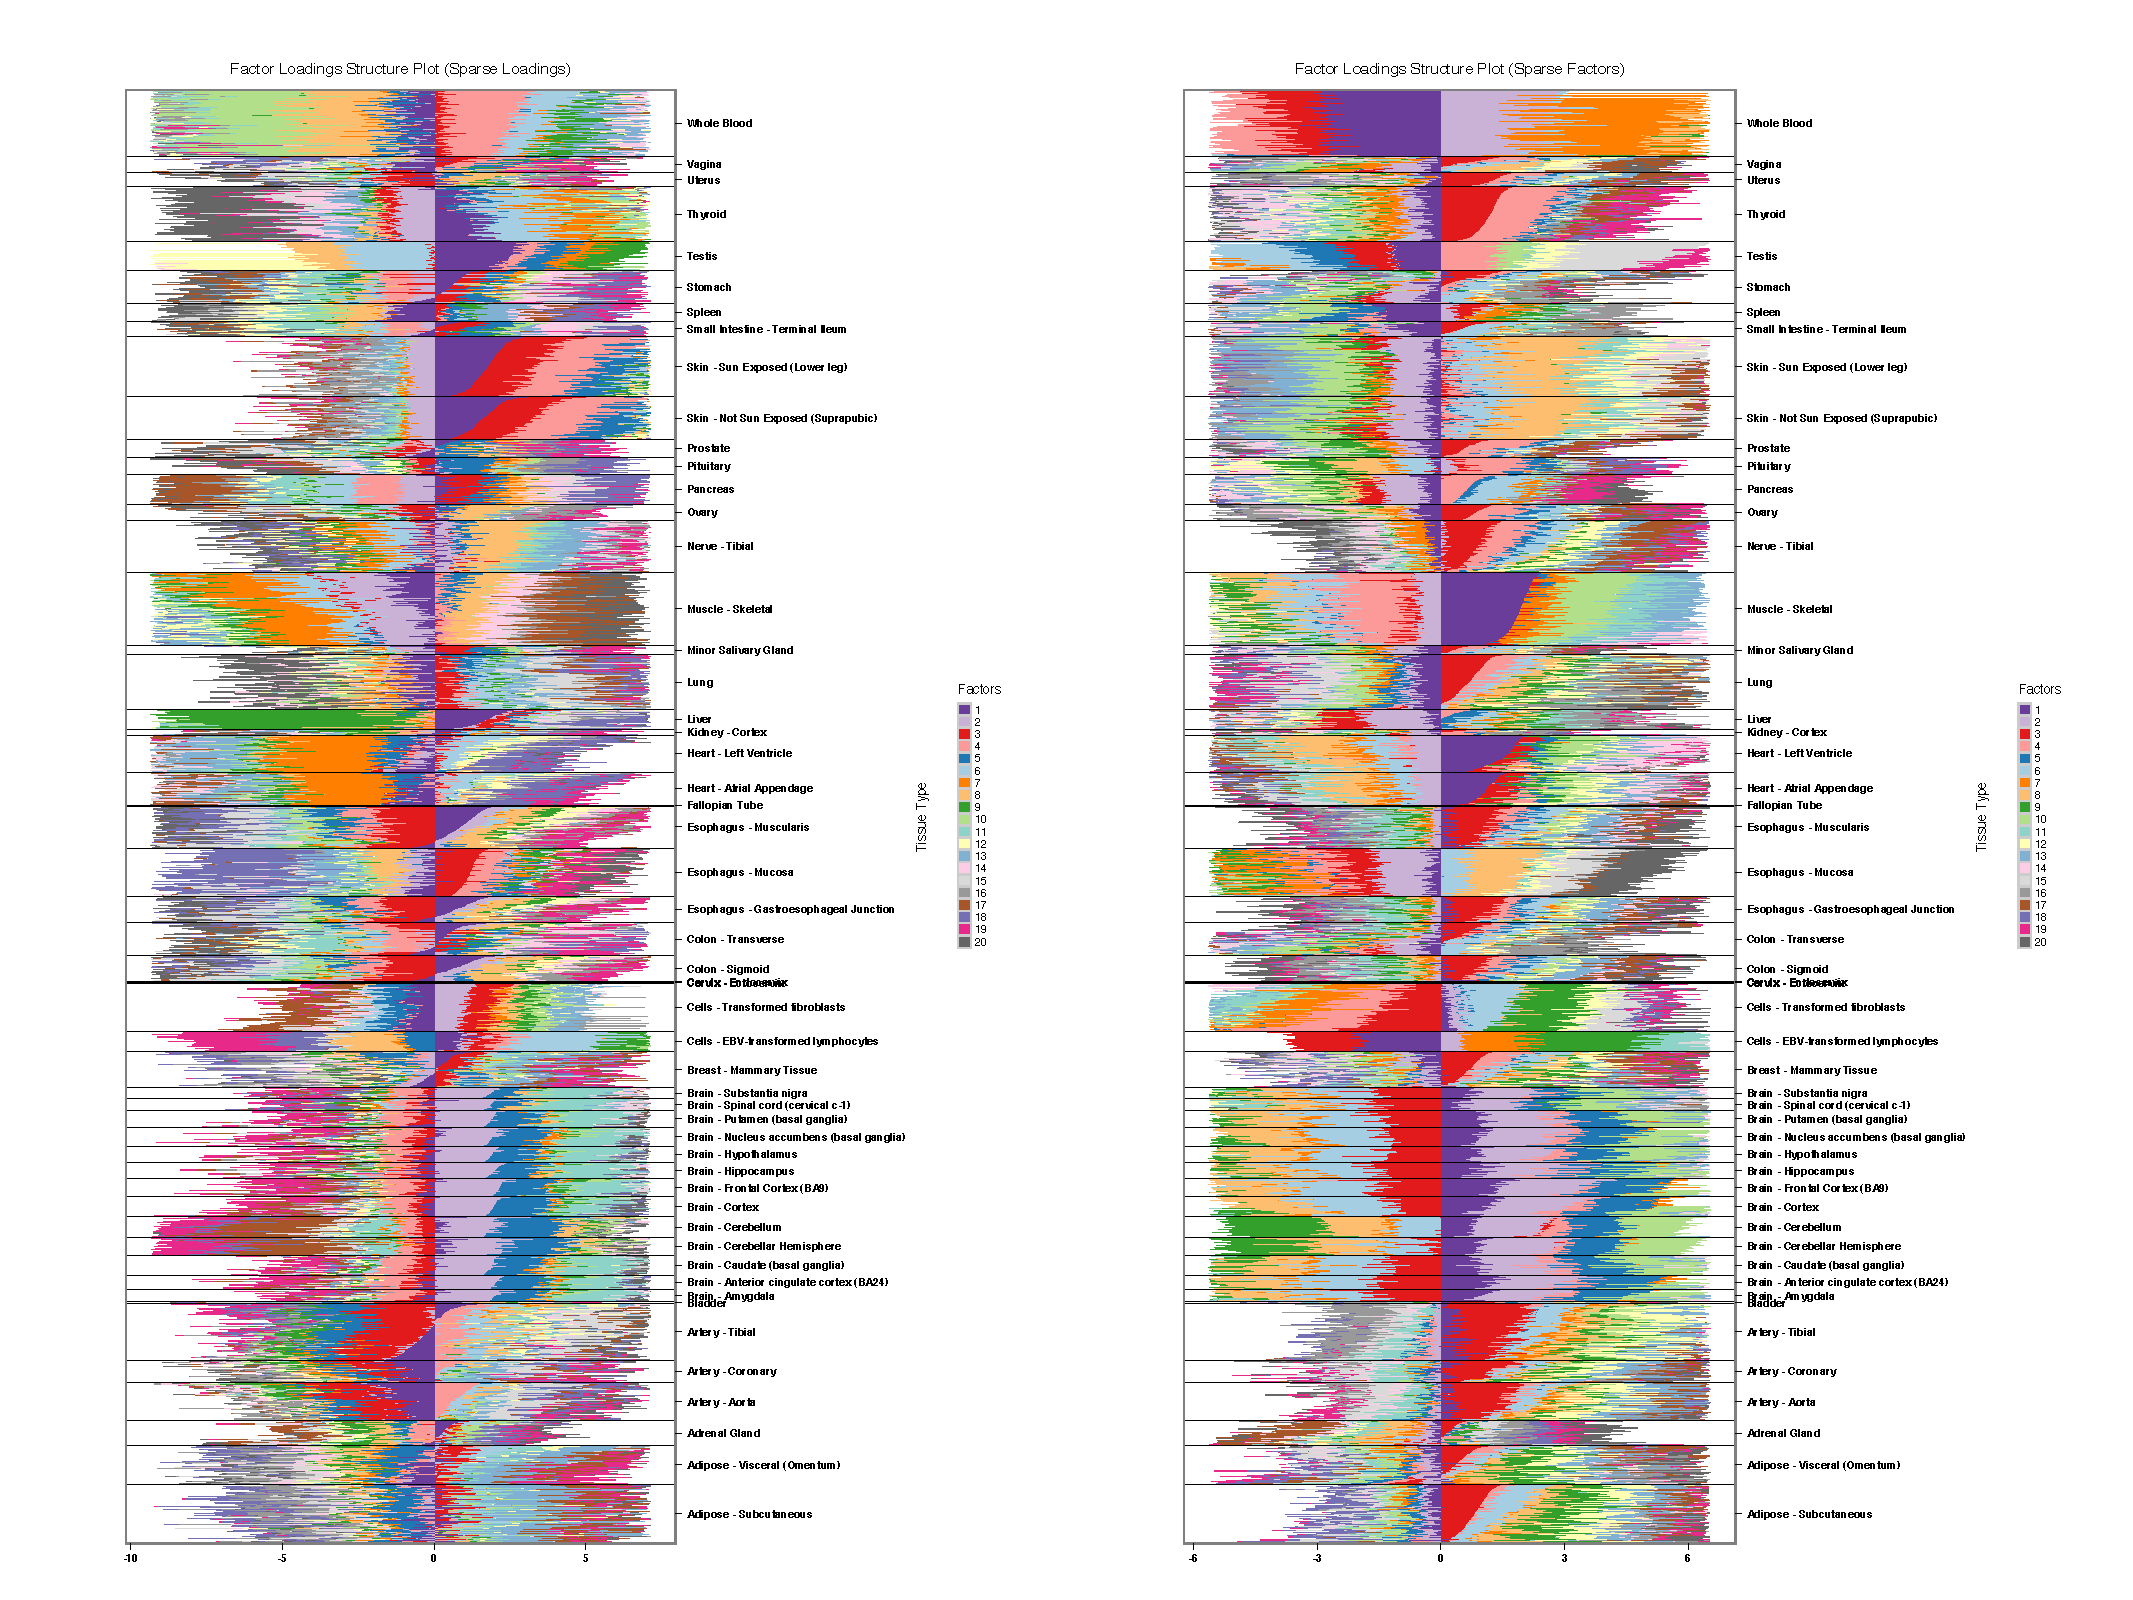
\includegraphics[height=6.3in, width=7in]{../../plots/gtex-figures/sfa_gtex_figs.png}
\end{figure}

\end{document}

\clearpage
% adopt PLoS genetics environment settings
\documentclass[10pt,letterpaper]{article}
\usepackage[top=0.85in,left=2.75in,footskip=0.75in]{geometry}

% Template for PLoS
% Version 3.2 March 2016

% General commands for the entire paper
%
% Use Unicode characters when possible
\usepackage[utf8x]{inputenc}
% amsmath package, useful for mathematical formulas
\usepackage{amsmath}
%\usepackage{natbib}
% amssymb package, useful for mathematical symbols
\usepackage{amssymb}
\usepackage{booktabs}
\usepackage{xspace}
\usepackage{hyperref}
% graphicx package, useful for including eps and pdf graphics
% include graphics with the command \includegraphics
\usepackage{graphicx}

% Use adjustwidth environment to exceed column width (see example table in text)
\usepackage{changepage}

% textcomp package and marvosym package for additional characters
\usepackage{textcomp,marvosym}

% fixltx2e package for \textsubscript
\usepackage{fixltx2e}

% cite package, to clean up citations in the main text. Do not remove.
\usepackage{cite}
\usepackage{caption}
\usepackage{subcaption}
\usepackage{rotating}

\usepackage{color}

% Use doublespacing - comment out for single spacing
%\usepackage{setspace}
%\doublespacing

% Text layout
\topmargin 0.0cm
\oddsidemargin 0.5cm
\evensidemargin 0.5cm
\textwidth 16cm
\textheight 21cm

\setlength{\parskip}{1em}

% Bold the 'Figure #' in the caption and separate it with a period
% Captions will be left justified
\usepackage[labelfont=bf,labelsep=period,justification=raggedright]{caption}

% Use the PLoS provided bibtex style
\bibliographystyle{/Users/stephens/Dropbox/Documents/stylefiles/plos2009}

% Remove brackets from numbering in List of References
\makeatletter
\renewcommand{\@biblabel}[1]{\quad#1.}
\makeatother

% Use nameref to cite supporting information files (see Supporting Information section for more info)
\usepackage{nameref,hyperref}

% line numbers
\usepackage[right]{lineno}

% ligatures disabled
\usepackage{microtype}
\DisableLigatures[f]{encoding = *, family = * }

% Leave date blank
\date{}

\pagestyle{myheadings}
%% ** EDIT HERE **
\usepackage{enumerate}
\usepackage{multirow}
\usepackage{url}
\usepackage{xr} %for cross-referencing
%% ** EDIT HERE **
%% PLEASE INCLUDE ALL MACROS BELOW
\newtheorem{algorithm}{Algorithm}
\newtheorem{proposition}{Proposition}
\newtheorem{restateproposition}{Proposition}
\newtheorem{lemma}{Lemma}
\newtheorem{corollary}{Corollary}
\newtheorem{result}{Result}
\newtheorem{note}{Note}
\newtheorem{definition}{Definition}

\def\KL{\text{KL}}


% Text layout
\raggedright
\setlength{\parindent}{0.5cm}
\textwidth 5.25in
\textheight 8.75in

% Bold the 'Figure #' in the caption and separate it from the title/caption with a period
% Captions will be left justified
\usepackage[aboveskip=1pt,labelfont=bf,labelsep=period,justification=raggedright,singlelinecheck=off]{caption}
\renewcommand{\figurename}{Fig}

%------ bibliography
% Use the PLoS provided BiBTeX style
\bibliographystyle{plos2015}
% Remove brackets from numbering in List of References
\makeatletter
\renewcommand{\@biblabel}[1]{\quad#1.}
\makeatother


% Header and Footer with logo
\usepackage{lastpage,fancyhdr,graphicx}
\usepackage{epstopdf}
\pagestyle{myheadings}
\pagestyle{fancy}
\fancyhf{}
\setlength{\headheight}{27.023pt}
\lhead{\includegraphics[width=2.0in]{PLOS-submission.eps}}
\rfoot{\thepage/\pageref{LastPage}}
\renewcommand{\footrule}{\hrule height 2pt \vspace{2mm}}
\fancyheadoffset[L]{2.25in}
\fancyfootoffset[L]{2.25in}
\lfoot{\sf PLOS}

%% Include all macros below

\newcommand{\lorem}{{\bf LOREM}}
\newcommand{\ipsum}{{\bf IPSUM}}

%% END MACROS SECTION

%% Author's settings
\def\KL{\text{KL}}


% Text layout specific to Supplemental Materials
\topmargin 0.0cm
\oddsidemargin 0.5cm
\evensidemargin 0.5cm
\textwidth 16cm
\textheight 21cm

\setlength{\parskip}{1em}

\begin{document}

\paragraph*{S7 Fig.}

\label{figS7}
{\bf GTEx brain tissue samples visualization using (A) principle component analysis, (B) t-SNE, and (C) Multidimensional scaling.}
The colors represent the 13 different brain tissue types. In (A) and (B), the majority of the tissue samples are distinct from Cerebellum tissue samples (the cluster of samples located on the right side of the plot). While, in (C), most tissue samples are located at the enter of the plot and are similar to each other in the t-SNE dimensions.

\begin{figure}[ht]
\centering
\includegraphics[height=4in, width=6in]{../../src/figure/gtex-brain-other-methods.Rmd/gtex-brain-with-legend.png}
\end{figure}

\end{document}

\clearpage
% adopt PLoS genetics environment settings
\documentclass[10pt,letterpaper]{article}
\usepackage[top=0.85in,left=2.75in,footskip=0.75in]{geometry}

% Template for PLoS
% Version 3.2 March 2016

% General commands for the entire paper
%
% Use Unicode characters when possible
\usepackage[utf8x]{inputenc}
% amsmath package, useful for mathematical formulas
\usepackage{amsmath}
%\usepackage{natbib}
% amssymb package, useful for mathematical symbols
\usepackage{amssymb}
\usepackage{booktabs}
\usepackage{xspace}
\usepackage{hyperref}
% graphicx package, useful for including eps and pdf graphics
% include graphics with the command \includegraphics
\usepackage{graphicx}

% Use adjustwidth environment to exceed column width (see example table in text)
\usepackage{changepage}

% textcomp package and marvosym package for additional characters
\usepackage{textcomp,marvosym}

% fixltx2e package for \textsubscript
\usepackage{fixltx2e}

% cite package, to clean up citations in the main text. Do not remove.
\usepackage{cite}
\usepackage{caption}
\usepackage{subcaption}
\usepackage{rotating}

\usepackage{color}

% Use doublespacing - comment out for single spacing
%\usepackage{setspace}
%\doublespacing

% Text layout
\topmargin 0.0cm
\oddsidemargin 0.5cm
\evensidemargin 0.5cm
\textwidth 16cm
\textheight 21cm

\setlength{\parskip}{1em}

% Bold the 'Figure #' in the caption and separate it with a period
% Captions will be left justified
\usepackage[labelfont=bf,labelsep=period,justification=raggedright]{caption}

% Use the PLoS provided bibtex style
\bibliographystyle{/Users/stephens/Dropbox/Documents/stylefiles/plos2009}

% Remove brackets from numbering in List of References
\makeatletter
\renewcommand{\@biblabel}[1]{\quad#1.}
\makeatother

% Use nameref to cite supporting information files (see Supporting Information section for more info)
\usepackage{nameref,hyperref}

% line numbers
\usepackage[right]{lineno}

% ligatures disabled
\usepackage{microtype}
\DisableLigatures[f]{encoding = *, family = * }

% Leave date blank
\date{}

\pagestyle{myheadings}
%% ** EDIT HERE **
\usepackage{enumerate}
\usepackage{multirow}
\usepackage{url}
\usepackage{xr} %for cross-referencing
%% ** EDIT HERE **
%% PLEASE INCLUDE ALL MACROS BELOW
\newtheorem{algorithm}{Algorithm}
\newtheorem{proposition}{Proposition}
\newtheorem{restateproposition}{Proposition}
\newtheorem{lemma}{Lemma}
\newtheorem{corollary}{Corollary}
\newtheorem{result}{Result}
\newtheorem{note}{Note}
\newtheorem{definition}{Definition}

\def\KL{\text{KL}}


% Text layout
\raggedright
\setlength{\parindent}{0.5cm}
\textwidth 5.25in
\textheight 8.75in

% Bold the 'Figure #' in the caption and separate it from the title/caption with a period
% Captions will be left justified
\usepackage[aboveskip=1pt,labelfont=bf,labelsep=period,justification=raggedright,singlelinecheck=off]{caption}
\renewcommand{\figurename}{Fig}

%------ bibliography
% Use the PLoS provided BiBTeX style
\bibliographystyle{plos2015}
% Remove brackets from numbering in List of References
\makeatletter
\renewcommand{\@biblabel}[1]{\quad#1.}
\makeatother


% Header and Footer with logo
\usepackage{lastpage,fancyhdr,graphicx}
\usepackage{epstopdf}
\pagestyle{myheadings}
\pagestyle{fancy}
\fancyhf{}
\setlength{\headheight}{27.023pt}
\lhead{\includegraphics[width=2.0in]{PLOS-submission.eps}}
\rfoot{\thepage/\pageref{LastPage}}
\renewcommand{\footrule}{\hrule height 2pt \vspace{2mm}}
\fancyheadoffset[L]{2.25in}
\fancyfootoffset[L]{2.25in}
\lfoot{\sf PLOS}

%% Include all macros below

\newcommand{\lorem}{{\bf LOREM}}
\newcommand{\ipsum}{{\bf IPSUM}}

%% END MACROS SECTION

%% Author's settings
\def\KL{\text{KL}}


% Text layout specific to Supplemental Materials
\topmargin 0.0cm
\oddsidemargin 0.5cm
\evensidemargin 0.5cm
\textwidth 16cm
\textheight 21cm

\setlength{\parskip}{1em}

\begin{document}

\paragraph*{S8 Fig.}

\label{figS8}
{\bf Dendrogram visualization of hierarchical clustering results of GTEx V6 tissue samples.} Hierarchical clustering of Euclidean distance based on complete linkage was applied to 8,555 tissue samples from the GTEx V6 data. Data was transformed to log counts per million (CPM) prior to clustering. Complete linkage method was used to plot the Dendrogram. The colors represent different tissue types. Samples from different tissues seem to cluster together, but any further patterns. However, because of the large number of samples, patterns of structural variation between tissue samples remain difficult to detect.
\begin{figure}[ht]
\centering
\includegraphics[height=6.3in, width=6in]{../../plots/dendextend_gtex.pdf}
\end{figure}

\end{document}

\clearpage
% adopt PLoS genetics environment settings
\documentclass[10pt,letterpaper]{article}
\usepackage[top=0.85in,left=2.75in,footskip=0.75in]{geometry}

% Template for PLoS
% Version 3.2 March 2016

% General commands for the entire paper
%
% Use Unicode characters when possible
\usepackage[utf8x]{inputenc}
% amsmath package, useful for mathematical formulas
\usepackage{amsmath}
%\usepackage{natbib}
% amssymb package, useful for mathematical symbols
\usepackage{amssymb}
\usepackage{booktabs}
\usepackage{xspace}
\usepackage{hyperref}
% graphicx package, useful for including eps and pdf graphics
% include graphics with the command \includegraphics
\usepackage{graphicx}

% Use adjustwidth environment to exceed column width (see example table in text)
\usepackage{changepage}

% textcomp package and marvosym package for additional characters
\usepackage{textcomp,marvosym}

% fixltx2e package for \textsubscript
\usepackage{fixltx2e}

% cite package, to clean up citations in the main text. Do not remove.
\usepackage{cite}
\usepackage{caption}
\usepackage{subcaption}
\usepackage{rotating}

\usepackage{color}

% Use doublespacing - comment out for single spacing
%\usepackage{setspace}
%\doublespacing

% Text layout
\topmargin 0.0cm
\oddsidemargin 0.5cm
\evensidemargin 0.5cm
\textwidth 16cm
\textheight 21cm

\setlength{\parskip}{1em}

% Bold the 'Figure #' in the caption and separate it with a period
% Captions will be left justified
\usepackage[labelfont=bf,labelsep=period,justification=raggedright]{caption}

% Use the PLoS provided bibtex style
\bibliographystyle{/Users/stephens/Dropbox/Documents/stylefiles/plos2009}

% Remove brackets from numbering in List of References
\makeatletter
\renewcommand{\@biblabel}[1]{\quad#1.}
\makeatother

% Use nameref to cite supporting information files (see Supporting Information section for more info)
\usepackage{nameref,hyperref}

% line numbers
\usepackage[right]{lineno}

% ligatures disabled
\usepackage{microtype}
\DisableLigatures[f]{encoding = *, family = * }

% Leave date blank
\date{}

\pagestyle{myheadings}
%% ** EDIT HERE **
\usepackage{enumerate}
\usepackage{multirow}
\usepackage{url}
\usepackage{xr} %for cross-referencing
%% ** EDIT HERE **
%% PLEASE INCLUDE ALL MACROS BELOW
\newtheorem{algorithm}{Algorithm}
\newtheorem{proposition}{Proposition}
\newtheorem{restateproposition}{Proposition}
\newtheorem{lemma}{Lemma}
\newtheorem{corollary}{Corollary}
\newtheorem{result}{Result}
\newtheorem{note}{Note}
\newtheorem{definition}{Definition}

\def\KL{\text{KL}}


% Text layout
\raggedright
\setlength{\parindent}{0.5cm}
\textwidth 5.25in
\textheight 8.75in

% Bold the 'Figure #' in the caption and separate it from the title/caption with a period
% Captions will be left justified
\usepackage[aboveskip=1pt,labelfont=bf,labelsep=period,justification=raggedright,singlelinecheck=off]{caption}
\renewcommand{\figurename}{Fig}

%------ bibliography
% Use the PLoS provided BiBTeX style
\bibliographystyle{plos2015}
% Remove brackets from numbering in List of References
\makeatletter
\renewcommand{\@biblabel}[1]{\quad#1.}
\makeatother


% Header and Footer with logo
\usepackage{lastpage,fancyhdr,graphicx}
\usepackage{epstopdf}
\pagestyle{myheadings}
\pagestyle{fancy}
\fancyhf{}
\setlength{\headheight}{27.023pt}
\lhead{\includegraphics[width=2.0in]{PLOS-submission.eps}}
\rfoot{\thepage/\pageref{LastPage}}
\renewcommand{\footrule}{\hrule height 2pt \vspace{2mm}}
\fancyheadoffset[L]{2.25in}
\fancyfootoffset[L]{2.25in}
\lfoot{\sf PLOS}

%% Include all macros below

\newcommand{\lorem}{{\bf LOREM}}
\newcommand{\ipsum}{{\bf IPSUM}}

%% END MACROS SECTION

%% Author's settings
\def\KL{\text{KL}}


% Text layout specific to Supplemental Materials
\topmargin 0.0cm
\oddsidemargin 0.5cm
\evensidemargin 0.5cm
\textwidth 16cm
\textheight 21cm

\setlength{\parskip}{1em}

\begin{document}

\paragraph*{S9 Fig.}

\label{figS9}
{\bf Hierarchical clustering results visualization of GTEx brain tissue samples.} Hierarchical clustering of Euclidean distance based on complete linkage was applied to 1,259 GTEx brain tissue samples. Data was transformed to log counts per million (CPM) prior to clustering. Complete linkage method was used to plot the Dendrogram. The colors represent different brain tissue types. We note that the sample labels in the Dendrogram are not easy to read because of the large sample size. However, there seems to be a separation between cerebellum, cerebellar hemisphere, spinal cord, and substantia nigra from other parts of the brain.

\begin{figure}[ht]
\centering
\includegraphics[height=6.3in, width=6in]{../../plots/dendextend_gtex_brain.pdf}
\end{figure}

\end{document}

\clearpage
% adopt PLoS genetics environment settings
\documentclass[10pt,letterpaper]{article}
\usepackage[top=0.85in,left=2.75in,footskip=0.75in]{geometry}

% Template for PLoS
% Version 3.2 March 2016

% General commands for the entire paper
%
% Use Unicode characters when possible
\usepackage[utf8x]{inputenc}
% amsmath package, useful for mathematical formulas
\usepackage{amsmath}
%\usepackage{natbib}
% amssymb package, useful for mathematical symbols
\usepackage{amssymb}
\usepackage{booktabs}
\usepackage{xspace}
\usepackage{hyperref}
% graphicx package, useful for including eps and pdf graphics
% include graphics with the command \includegraphics
\usepackage{graphicx}

% Use adjustwidth environment to exceed column width (see example table in text)
\usepackage{changepage}

% textcomp package and marvosym package for additional characters
\usepackage{textcomp,marvosym}

% fixltx2e package for \textsubscript
\usepackage{fixltx2e}

% cite package, to clean up citations in the main text. Do not remove.
\usepackage{cite}
\usepackage{caption}
\usepackage{subcaption}
\usepackage{rotating}

\usepackage{color}

% Use doublespacing - comment out for single spacing
%\usepackage{setspace}
%\doublespacing

% Text layout
\topmargin 0.0cm
\oddsidemargin 0.5cm
\evensidemargin 0.5cm
\textwidth 16cm
\textheight 21cm

\setlength{\parskip}{1em}

% Bold the 'Figure #' in the caption and separate it with a period
% Captions will be left justified
\usepackage[labelfont=bf,labelsep=period,justification=raggedright]{caption}

% Use the PLoS provided bibtex style
\bibliographystyle{/Users/stephens/Dropbox/Documents/stylefiles/plos2009}

% Remove brackets from numbering in List of References
\makeatletter
\renewcommand{\@biblabel}[1]{\quad#1.}
\makeatother

% Use nameref to cite supporting information files (see Supporting Information section for more info)
\usepackage{nameref,hyperref}

% line numbers
\usepackage[right]{lineno}

% ligatures disabled
\usepackage{microtype}
\DisableLigatures[f]{encoding = *, family = * }

% Leave date blank
\date{}

\pagestyle{myheadings}
%% ** EDIT HERE **
\usepackage{enumerate}
\usepackage{multirow}
\usepackage{url}
\usepackage{xr} %for cross-referencing
%% ** EDIT HERE **
%% PLEASE INCLUDE ALL MACROS BELOW
\newtheorem{algorithm}{Algorithm}
\newtheorem{proposition}{Proposition}
\newtheorem{restateproposition}{Proposition}
\newtheorem{lemma}{Lemma}
\newtheorem{corollary}{Corollary}
\newtheorem{result}{Result}
\newtheorem{note}{Note}
\newtheorem{definition}{Definition}

\def\KL{\text{KL}}


% Text layout
\raggedright
\setlength{\parindent}{0.5cm}
\textwidth 5.25in
\textheight 8.75in

% Bold the 'Figure #' in the caption and separate it from the title/caption with a period
% Captions will be left justified
\usepackage[aboveskip=1pt,labelfont=bf,labelsep=period,justification=raggedright,singlelinecheck=off]{caption}
\renewcommand{\figurename}{Fig}

%------ bibliography
% Use the PLoS provided BiBTeX style
\bibliographystyle{plos2015}
% Remove brackets from numbering in List of References
\makeatletter
\renewcommand{\@biblabel}[1]{\quad#1.}
\makeatother


% Header and Footer with logo
\usepackage{lastpage,fancyhdr,graphicx}
\usepackage{epstopdf}
\pagestyle{myheadings}
\pagestyle{fancy}
\fancyhf{}
\setlength{\headheight}{27.023pt}
\lhead{\includegraphics[width=2.0in]{PLOS-submission.eps}}
\rfoot{\thepage/\pageref{LastPage}}
\renewcommand{\footrule}{\hrule height 2pt \vspace{2mm}}
\fancyheadoffset[L]{2.25in}
\fancyfootoffset[L]{2.25in}
\lfoot{\sf PLOS}

%% Include all macros below

\newcommand{\lorem}{{\bf LOREM}}
\newcommand{\ipsum}{{\bf IPSUM}}

%% END MACROS SECTION

%% Author's settings
\def\KL{\text{KL}}


% Text layout specific to Supplemental Materials
\topmargin 0.0cm
\oddsidemargin 0.5cm
\evensidemargin 0.5cm
\textwidth 16cm
\textheight 21cm

\setlength{\parskip}{1em}

\begin{document}

\paragraph*{S10 Fig.}

\label{figS10}
{\bf Dendrogram visualization of hierarchical clustering results of mouse pre-implantation embryos data from Deng et al (2014).} Hierarchical clustering of Euclidean distance based on complete linkage was applied to 259 single cell samples from Deng et al., (2014). Data was transformed to log counts per million (CPM) prior to clustering. The colors represent different developmental phases. Although samples from different developmental stages seem to cluster together, the samples are not arranged in a continuum according to their developmental stages.
\begin{figure}[ht]
\centering
\includegraphics[height=6.3in, width=6in]{../../plots/dendextend_deng.pdf}
\end{figure}

\end{document}

\clearpage
% adopt PLoS genetics environment settings
\documentclass[10pt,letterpaper]{article}
\usepackage[top=0.85in,left=2.75in,footskip=0.75in]{geometry}

% Template for PLoS
% Version 3.2 March 2016

% General commands for the entire paper
%
% Use Unicode characters when possible
\usepackage[utf8x]{inputenc}
% amsmath package, useful for mathematical formulas
\usepackage{amsmath}
%\usepackage{natbib}
% amssymb package, useful for mathematical symbols
\usepackage{amssymb}
\usepackage{booktabs}
\usepackage{xspace}
\usepackage{hyperref}
% graphicx package, useful for including eps and pdf graphics
% include graphics with the command \includegraphics
\usepackage{graphicx}

% Use adjustwidth environment to exceed column width (see example table in text)
\usepackage{changepage}

% textcomp package and marvosym package for additional characters
\usepackage{textcomp,marvosym}

% fixltx2e package for \textsubscript
\usepackage{fixltx2e}

% cite package, to clean up citations in the main text. Do not remove.
\usepackage{cite}
\usepackage{caption}
\usepackage{subcaption}
\usepackage{rotating}

\usepackage{color}

% Use doublespacing - comment out for single spacing
%\usepackage{setspace}
%\doublespacing

% Text layout
\topmargin 0.0cm
\oddsidemargin 0.5cm
\evensidemargin 0.5cm
\textwidth 16cm
\textheight 21cm

\setlength{\parskip}{1em}

% Bold the 'Figure #' in the caption and separate it with a period
% Captions will be left justified
\usepackage[labelfont=bf,labelsep=period,justification=raggedright]{caption}

% Use the PLoS provided bibtex style
\bibliographystyle{/Users/stephens/Dropbox/Documents/stylefiles/plos2009}

% Remove brackets from numbering in List of References
\makeatletter
\renewcommand{\@biblabel}[1]{\quad#1.}
\makeatother

% Use nameref to cite supporting information files (see Supporting Information section for more info)
\usepackage{nameref,hyperref}

% line numbers
\usepackage[right]{lineno}

% ligatures disabled
\usepackage{microtype}
\DisableLigatures[f]{encoding = *, family = * }

% Leave date blank
\date{}

\pagestyle{myheadings}
%% ** EDIT HERE **
\usepackage{enumerate}
\usepackage{multirow}
\usepackage{url}
\usepackage{xr} %for cross-referencing
%% ** EDIT HERE **
%% PLEASE INCLUDE ALL MACROS BELOW
\newtheorem{algorithm}{Algorithm}
\newtheorem{proposition}{Proposition}
\newtheorem{restateproposition}{Proposition}
\newtheorem{lemma}{Lemma}
\newtheorem{corollary}{Corollary}
\newtheorem{result}{Result}
\newtheorem{note}{Note}
\newtheorem{definition}{Definition}

\def\KL{\text{KL}}


% Text layout
\raggedright
\setlength{\parindent}{0.5cm}
\textwidth 5.25in
\textheight 8.75in

% Bold the 'Figure #' in the caption and separate it from the title/caption with a period
% Captions will be left justified
\usepackage[aboveskip=1pt,labelfont=bf,labelsep=period,justification=raggedright,singlelinecheck=off]{caption}
\renewcommand{\figurename}{Fig}

%------ bibliography
% Use the PLoS provided BiBTeX style
\bibliographystyle{plos2015}
% Remove brackets from numbering in List of References
\makeatletter
\renewcommand{\@biblabel}[1]{\quad#1.}
\makeatother


% Header and Footer with logo
\usepackage{lastpage,fancyhdr,graphicx}
\usepackage{epstopdf}
\pagestyle{myheadings}
\pagestyle{fancy}
\fancyhf{}
\setlength{\headheight}{27.023pt}
\lhead{\includegraphics[width=2.0in]{PLOS-submission.eps}}
\rfoot{\thepage/\pageref{LastPage}}
\renewcommand{\footrule}{\hrule height 2pt \vspace{2mm}}
\fancyheadoffset[L]{2.25in}
\fancyfootoffset[L]{2.25in}
\lfoot{\sf PLOS}

%% Include all macros below

\newcommand{\lorem}{{\bf LOREM}}
\newcommand{\ipsum}{{\bf IPSUM}}

%% END MACROS SECTION

%% Author's settings
\def\KL{\text{KL}}


\begin{document}

\paragraph*{S11 Fig.}

\label{figS11}
{\bf Dendogram representation for GTEx Brain tissue level data.
\begin{figure}[ht]
\centering
\includegraphics[height=6.3in, width=7in]{../../plots/dendextend_gtex_brain.pdf}
\caption{Dendogram representation of the 1259 GTEx brain tissue samples. 
The hierarchical clustering in this case has been performed on the log counts per million (cpm) data. 
Note that the labels in this case are not visible because of large sample size but largely it separates out
Brain Cerebellar, Cerebellar hemisphere  and Brain Spinal Cord, Substantia Nigra from other parts of the brain. But any other structure in the data is not easy to see or interpret.}
\end{figure}

\end{document}
\clearpage
% adopt PLoS genetics environment settings
\documentclass[10pt,letterpaper]{article}
\usepackage[top=0.85in,left=2.75in,footskip=0.75in]{geometry}

% Template for PLoS
% Version 3.2 March 2016

% General commands for the entire paper
%
% Use Unicode characters when possible
\usepackage[utf8x]{inputenc}
% amsmath package, useful for mathematical formulas
\usepackage{amsmath}
%\usepackage{natbib}
% amssymb package, useful for mathematical symbols
\usepackage{amssymb}
\usepackage{booktabs}
\usepackage{xspace}
\usepackage{hyperref}
% graphicx package, useful for including eps and pdf graphics
% include graphics with the command \includegraphics
\usepackage{graphicx}

% Use adjustwidth environment to exceed column width (see example table in text)
\usepackage{changepage}

% textcomp package and marvosym package for additional characters
\usepackage{textcomp,marvosym}

% fixltx2e package for \textsubscript
\usepackage{fixltx2e}

% cite package, to clean up citations in the main text. Do not remove.
\usepackage{cite}
\usepackage{caption}
\usepackage{subcaption}
\usepackage{rotating}

\usepackage{color}

% Use doublespacing - comment out for single spacing
%\usepackage{setspace}
%\doublespacing

% Text layout
\topmargin 0.0cm
\oddsidemargin 0.5cm
\evensidemargin 0.5cm
\textwidth 16cm
\textheight 21cm

\setlength{\parskip}{1em}

% Bold the 'Figure #' in the caption and separate it with a period
% Captions will be left justified
\usepackage[labelfont=bf,labelsep=period,justification=raggedright]{caption}

% Use the PLoS provided bibtex style
\bibliographystyle{/Users/stephens/Dropbox/Documents/stylefiles/plos2009}

% Remove brackets from numbering in List of References
\makeatletter
\renewcommand{\@biblabel}[1]{\quad#1.}
\makeatother

% Use nameref to cite supporting information files (see Supporting Information section for more info)
\usepackage{nameref,hyperref}

% line numbers
\usepackage[right]{lineno}

% ligatures disabled
\usepackage{microtype}
\DisableLigatures[f]{encoding = *, family = * }

% Leave date blank
\date{}

\pagestyle{myheadings}
%% ** EDIT HERE **
\usepackage{enumerate}
\usepackage{multirow}
\usepackage{url}
\usepackage{xr} %for cross-referencing
%% ** EDIT HERE **
%% PLEASE INCLUDE ALL MACROS BELOW
\newtheorem{algorithm}{Algorithm}
\newtheorem{proposition}{Proposition}
\newtheorem{restateproposition}{Proposition}
\newtheorem{lemma}{Lemma}
\newtheorem{corollary}{Corollary}
\newtheorem{result}{Result}
\newtheorem{note}{Note}
\newtheorem{definition}{Definition}

\def\KL{\text{KL}}


% Text layout
\raggedright
\setlength{\parindent}{0.5cm}
\textwidth 5.25in
\textheight 8.75in

% Bold the 'Figure #' in the caption and separate it from the title/caption with a period
% Captions will be left justified
\usepackage[aboveskip=1pt,labelfont=bf,labelsep=period,justification=raggedright,singlelinecheck=off]{caption}
\renewcommand{\figurename}{Fig}

%------ bibliography
% Use the PLoS provided BiBTeX style
\bibliographystyle{plos2015}
% Remove brackets from numbering in List of References
\makeatletter
\renewcommand{\@biblabel}[1]{\quad#1.}
\makeatother


% Header and Footer with logo
\usepackage{lastpage,fancyhdr,graphicx}
\usepackage{epstopdf}
\pagestyle{myheadings}
\pagestyle{fancy}
\fancyhf{}
\setlength{\headheight}{27.023pt}
\lhead{\includegraphics[width=2.0in]{PLOS-submission.eps}}
\rfoot{\thepage/\pageref{LastPage}}
\renewcommand{\footrule}{\hrule height 2pt \vspace{2mm}}
\fancyheadoffset[L]{2.25in}
\fancyfootoffset[L]{2.25in}
\lfoot{\sf PLOS}

%% Include all macros below

\newcommand{\lorem}{{\bf LOREM}}
\newcommand{\ipsum}{{\bf IPSUM}}

%% END MACROS SECTION

%% Author's settings
\def\KL{\text{KL}}


% Text layout specific to Supplemental Materials
\topmargin 0.0cm
\oddsidemargin 0.5cm
\evensidemargin 0.5cm
\textwidth 16cm
\textheight 21cm

\setlength{\parskip}{1em}

\begin{document}

\paragraph*{S12 Fig.}

\label{figS12}
{\bf Dendrogram representation for GTEx all tissues level data.} Dendrogram representation of the 8555 GTEx tissue samples across all the tissues.
The hierarchical clustering in this case has been performed on the log counts per million (cpm) data.
Very clearly, samples from different tissues seem to cluster together, but any further patterns, for instance, how similar different tissue types are, is hard to see.
\begin{figure}[ht]
\centering
\includegraphics[height=6.3in, width=6in]{../../plots/dendextend_gtex.pdf}
\end{figure}

\end{document}

\clearpage
% adopt PLoS genetics environment settings
\documentclass[10pt,letterpaper]{article}
\usepackage[top=0.85in,left=2.75in,footskip=0.75in]{geometry}

% Template for PLoS
% Version 3.2 March 2016

% General commands for the entire paper
%
% Use Unicode characters when possible
\usepackage[utf8x]{inputenc}
% amsmath package, useful for mathematical formulas
\usepackage{amsmath}
%\usepackage{natbib}
% amssymb package, useful for mathematical symbols
\usepackage{amssymb}
\usepackage{booktabs}
\usepackage{xspace}
\usepackage{hyperref}
% graphicx package, useful for including eps and pdf graphics
% include graphics with the command \includegraphics
\usepackage{graphicx}

% Use adjustwidth environment to exceed column width (see example table in text)
\usepackage{changepage}

% textcomp package and marvosym package for additional characters
\usepackage{textcomp,marvosym}

% fixltx2e package for \textsubscript
\usepackage{fixltx2e}

% cite package, to clean up citations in the main text. Do not remove.
\usepackage{cite}
\usepackage{caption}
\usepackage{subcaption}
\usepackage{rotating}

\usepackage{color}

% Use doublespacing - comment out for single spacing
%\usepackage{setspace}
%\doublespacing

% Text layout
\topmargin 0.0cm
\oddsidemargin 0.5cm
\evensidemargin 0.5cm
\textwidth 16cm
\textheight 21cm

\setlength{\parskip}{1em}

% Bold the 'Figure #' in the caption and separate it with a period
% Captions will be left justified
\usepackage[labelfont=bf,labelsep=period,justification=raggedright]{caption}

% Use the PLoS provided bibtex style
\bibliographystyle{/Users/stephens/Dropbox/Documents/stylefiles/plos2009}

% Remove brackets from numbering in List of References
\makeatletter
\renewcommand{\@biblabel}[1]{\quad#1.}
\makeatother

% Use nameref to cite supporting information files (see Supporting Information section for more info)
\usepackage{nameref,hyperref}

% line numbers
\usepackage[right]{lineno}

% ligatures disabled
\usepackage{microtype}
\DisableLigatures[f]{encoding = *, family = * }

% Leave date blank
\date{}

\pagestyle{myheadings}
%% ** EDIT HERE **
\usepackage{enumerate}
\usepackage{multirow}
\usepackage{url}
\usepackage{xr} %for cross-referencing
%% ** EDIT HERE **
%% PLEASE INCLUDE ALL MACROS BELOW
\newtheorem{algorithm}{Algorithm}
\newtheorem{proposition}{Proposition}
\newtheorem{restateproposition}{Proposition}
\newtheorem{lemma}{Lemma}
\newtheorem{corollary}{Corollary}
\newtheorem{result}{Result}
\newtheorem{note}{Note}
\newtheorem{definition}{Definition}

\def\KL{\text{KL}}


% Text layout
\raggedright
\setlength{\parindent}{0.5cm}
\textwidth 5.25in
\textheight 8.75in

% Bold the 'Figure #' in the caption and separate it from the title/caption with a period
% Captions will be left justified
\usepackage[aboveskip=1pt,labelfont=bf,labelsep=period,justification=raggedright,singlelinecheck=off]{caption}
\renewcommand{\figurename}{Fig}

%------ bibliography
% Use the PLoS provided BiBTeX style
\bibliographystyle{plos2015}
% Remove brackets from numbering in List of References
\makeatletter
\renewcommand{\@biblabel}[1]{\quad#1.}
\makeatother


% Header and Footer with logo
\usepackage{lastpage,fancyhdr,graphicx}
\usepackage{epstopdf}
\pagestyle{myheadings}
\pagestyle{fancy}
\fancyhf{}
\setlength{\headheight}{27.023pt}
\lhead{\includegraphics[width=2.0in]{PLOS-submission.eps}}
\rfoot{\thepage/\pageref{LastPage}}
\renewcommand{\footrule}{\hrule height 2pt \vspace{2mm}}
\fancyheadoffset[L]{2.25in}
\fancyfootoffset[L]{2.25in}
\lfoot{\sf PLOS}

%% Include all macros below

\newcommand{\lorem}{{\bf LOREM}}
\newcommand{\ipsum}{{\bf IPSUM}}

%% END MACROS SECTION

%% Author's settings
\def\KL{\text{KL}}


% Text layout specific to Supplemental Materials
\topmargin 0.0cm
\oddsidemargin 0.5cm
\evensidemargin 0.5cm
\textwidth 16cm
\textheight 21cm

\setlength{\parskip}{1em}

\begin{document}

\paragraph*{S13 Fig.}

\label{figS13}
{\bf Top oder PC scatter plots for GTEx V6 all tissues data.}
\begin{figure}[ht]
\centering
\includegraphics[height=6in, width=6in]{../../plots/gtex-figures/gtex-high-pcs.pdf}
\caption{Scatter plot representation of the different top order PCs of the GTEx samples based on the RNa-seq expression data (log cpm normalized).}
\end{figure}

\end{document}

\clearpage
% adopt PLoS genetics environment settings
\documentclass[10pt,letterpaper]{article}
\usepackage[top=0.85in,left=2.75in,footskip=0.75in]{geometry}

% Template for PLoS
% Version 3.2 March 2016

% General commands for the entire paper
%
% Use Unicode characters when possible
\usepackage[utf8x]{inputenc}
% amsmath package, useful for mathematical formulas
\usepackage{amsmath}
%\usepackage{natbib}
% amssymb package, useful for mathematical symbols
\usepackage{amssymb}
\usepackage{booktabs}
\usepackage{xspace}
\usepackage{hyperref}
% graphicx package, useful for including eps and pdf graphics
% include graphics with the command \includegraphics
\usepackage{graphicx}

% Use adjustwidth environment to exceed column width (see example table in text)
\usepackage{changepage}

% textcomp package and marvosym package for additional characters
\usepackage{textcomp,marvosym}

% fixltx2e package for \textsubscript
\usepackage{fixltx2e}

% cite package, to clean up citations in the main text. Do not remove.
\usepackage{cite}
\usepackage{caption}
\usepackage{subcaption}
\usepackage{rotating}

\usepackage{color}

% Use doublespacing - comment out for single spacing
%\usepackage{setspace}
%\doublespacing

% Text layout
\topmargin 0.0cm
\oddsidemargin 0.5cm
\evensidemargin 0.5cm
\textwidth 16cm
\textheight 21cm

\setlength{\parskip}{1em}

% Bold the 'Figure #' in the caption and separate it with a period
% Captions will be left justified
\usepackage[labelfont=bf,labelsep=period,justification=raggedright]{caption}

% Use the PLoS provided bibtex style
\bibliographystyle{/Users/stephens/Dropbox/Documents/stylefiles/plos2009}

% Remove brackets from numbering in List of References
\makeatletter
\renewcommand{\@biblabel}[1]{\quad#1.}
\makeatother

% Use nameref to cite supporting information files (see Supporting Information section for more info)
\usepackage{nameref,hyperref}

% line numbers
\usepackage[right]{lineno}

% ligatures disabled
\usepackage{microtype}
\DisableLigatures[f]{encoding = *, family = * }

% Leave date blank
\date{}

\pagestyle{myheadings}
%% ** EDIT HERE **
\usepackage{enumerate}
\usepackage{multirow}
\usepackage{url}
\usepackage{xr} %for cross-referencing
%% ** EDIT HERE **
%% PLEASE INCLUDE ALL MACROS BELOW
\newtheorem{algorithm}{Algorithm}
\newtheorem{proposition}{Proposition}
\newtheorem{restateproposition}{Proposition}
\newtheorem{lemma}{Lemma}
\newtheorem{corollary}{Corollary}
\newtheorem{result}{Result}
\newtheorem{note}{Note}
\newtheorem{definition}{Definition}

\def\KL{\text{KL}}


% Text layout
\raggedright
\setlength{\parindent}{0.5cm}
\textwidth 5.25in
\textheight 8.75in

% Bold the 'Figure #' in the caption and separate it from the title/caption with a period
% Captions will be left justified
\usepackage[aboveskip=1pt,labelfont=bf,labelsep=period,justification=raggedright,singlelinecheck=off]{caption}
\renewcommand{\figurename}{Fig}

%------ bibliography
% Use the PLoS provided BiBTeX style
\bibliographystyle{plos2015}
% Remove brackets from numbering in List of References
\makeatletter
\renewcommand{\@biblabel}[1]{\quad#1.}
\makeatother


% Header and Footer with logo
\usepackage{lastpage,fancyhdr,graphicx}
\usepackage{epstopdf}
\pagestyle{myheadings}
\pagestyle{fancy}
\fancyhf{}
\setlength{\headheight}{27.023pt}
\lhead{\includegraphics[width=2.0in]{PLOS-submission.eps}}
\rfoot{\thepage/\pageref{LastPage}}
\renewcommand{\footrule}{\hrule height 2pt \vspace{2mm}}
\fancyheadoffset[L]{2.25in}
\fancyfootoffset[L]{2.25in}
\lfoot{\sf PLOS}

%% Include all macros below

\newcommand{\lorem}{{\bf LOREM}}
\newcommand{\ipsum}{{\bf IPSUM}}

%% END MACROS SECTION

%% Author's settings
\def\KL{\text{KL}}


% Text layout specific to Supplemental Materials
\topmargin 0.0cm
\oddsidemargin 0.5cm
\evensidemargin 0.5cm
\textwidth 16cm
\textheight 21cm

\setlength{\parskip}{1em}

\begin{document}

\paragraph*{S14 Fig.}

\label{figS14}
{\bf Sparse Factor Analysis loadings visualization of GTEx V6 tissue samples.} The colors represent the 20 different factors. The factor loadings are presented in a stacked bar for each sample. We performed SFA under the scenarios of (A) when the loadings are sparse and (B) when the factors are sparse.
\begin{figure}[ht]
\centering
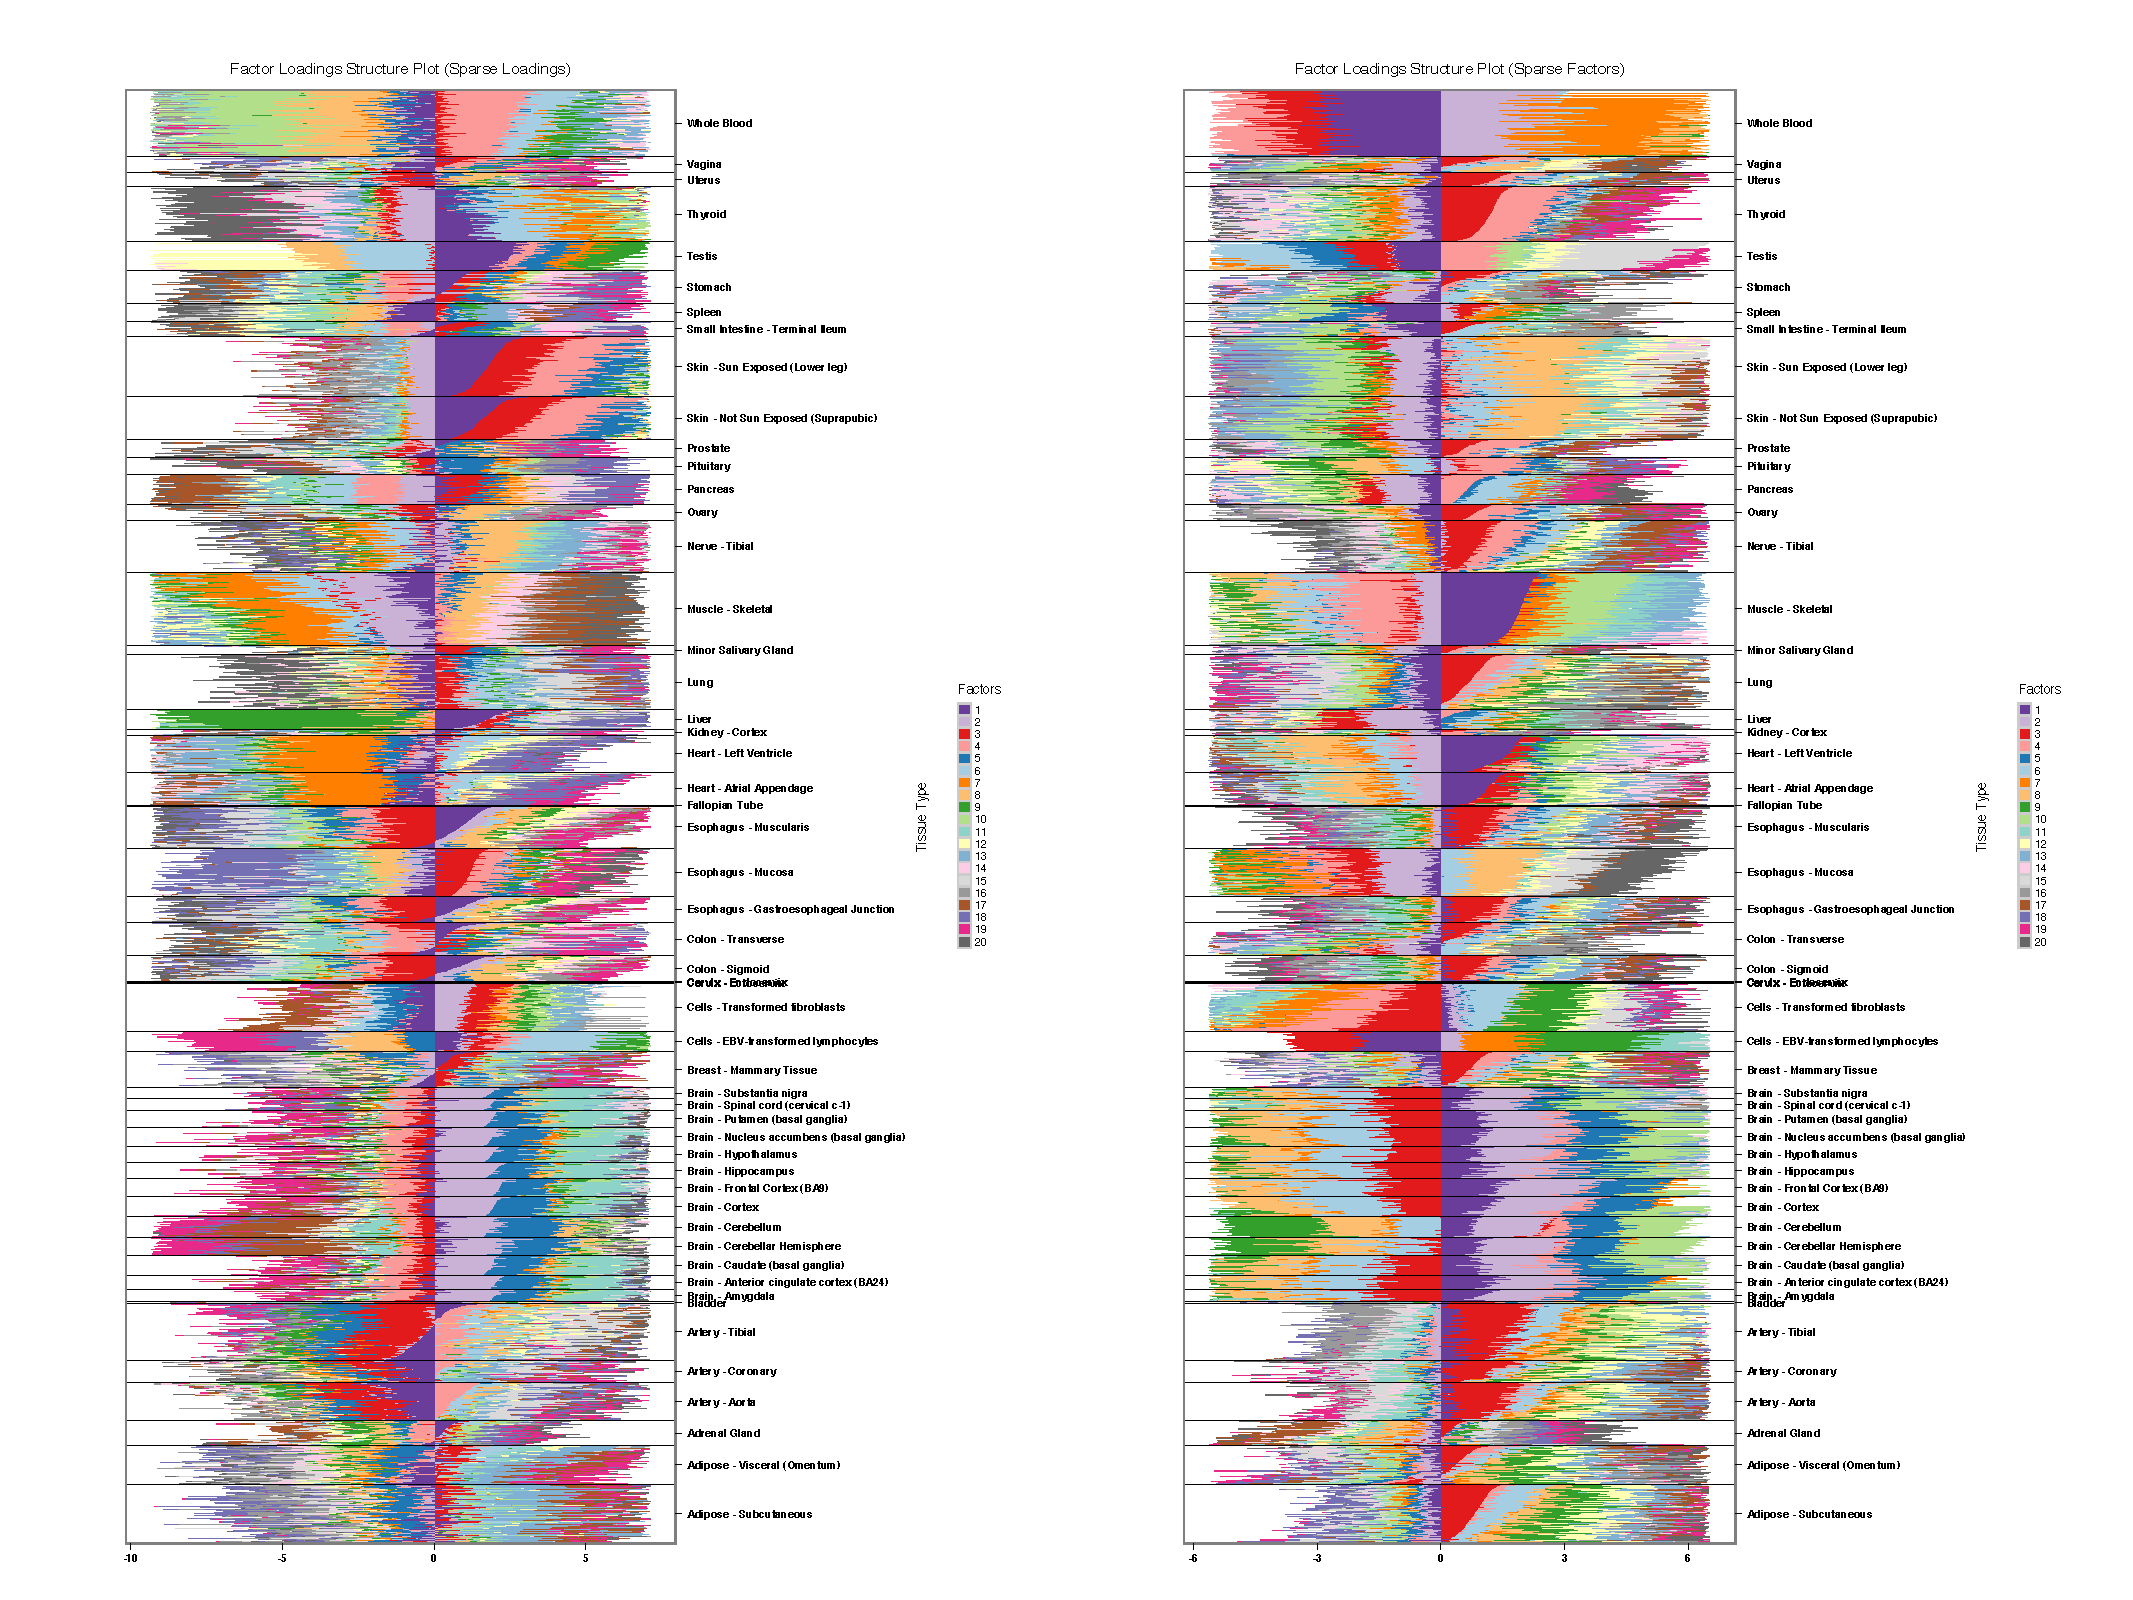
\includegraphics[height=6.3in, width=7in]{../../plots/gtex-figures/sfa_gtex_figs.png}
\end{figure}

\end{document}

\clearpage
% adopt PLoS genetics environment settings
\documentclass[10pt,letterpaper]{article}
\usepackage[top=0.85in,left=2.75in,footskip=0.75in]{geometry}

% Template for PLoS
% Version 3.2 March 2016

% General commands for the entire paper
%
% Use Unicode characters when possible
\usepackage[utf8x]{inputenc}
% amsmath package, useful for mathematical formulas
\usepackage{amsmath}
%\usepackage{natbib}
% amssymb package, useful for mathematical symbols
\usepackage{amssymb}
\usepackage{booktabs}
\usepackage{xspace}
\usepackage{hyperref}
% graphicx package, useful for including eps and pdf graphics
% include graphics with the command \includegraphics
\usepackage{graphicx}

% Use adjustwidth environment to exceed column width (see example table in text)
\usepackage{changepage}

% textcomp package and marvosym package for additional characters
\usepackage{textcomp,marvosym}

% fixltx2e package for \textsubscript
\usepackage{fixltx2e}

% cite package, to clean up citations in the main text. Do not remove.
\usepackage{cite}
\usepackage{caption}
\usepackage{subcaption}
\usepackage{rotating}

\usepackage{color}

% Use doublespacing - comment out for single spacing
%\usepackage{setspace}
%\doublespacing

% Text layout
\topmargin 0.0cm
\oddsidemargin 0.5cm
\evensidemargin 0.5cm
\textwidth 16cm
\textheight 21cm

\setlength{\parskip}{1em}

% Bold the 'Figure #' in the caption and separate it with a period
% Captions will be left justified
\usepackage[labelfont=bf,labelsep=period,justification=raggedright]{caption}

% Use the PLoS provided bibtex style
\bibliographystyle{/Users/stephens/Dropbox/Documents/stylefiles/plos2009}

% Remove brackets from numbering in List of References
\makeatletter
\renewcommand{\@biblabel}[1]{\quad#1.}
\makeatother

% Use nameref to cite supporting information files (see Supporting Information section for more info)
\usepackage{nameref,hyperref}

% line numbers
\usepackage[right]{lineno}

% ligatures disabled
\usepackage{microtype}
\DisableLigatures[f]{encoding = *, family = * }

% Leave date blank
\date{}

\pagestyle{myheadings}
%% ** EDIT HERE **
\usepackage{enumerate}
\usepackage{multirow}
\usepackage{url}
\usepackage{xr} %for cross-referencing
%% ** EDIT HERE **
%% PLEASE INCLUDE ALL MACROS BELOW
\newtheorem{algorithm}{Algorithm}
\newtheorem{proposition}{Proposition}
\newtheorem{restateproposition}{Proposition}
\newtheorem{lemma}{Lemma}
\newtheorem{corollary}{Corollary}
\newtheorem{result}{Result}
\newtheorem{note}{Note}
\newtheorem{definition}{Definition}

\def\KL{\text{KL}}


% Text layout
\raggedright
\setlength{\parindent}{0.5cm}
\textwidth 5.25in
\textheight 8.75in

% Bold the 'Figure #' in the caption and separate it from the title/caption with a period
% Captions will be left justified
\usepackage[aboveskip=1pt,labelfont=bf,labelsep=period,justification=raggedright,singlelinecheck=off]{caption}
\renewcommand{\figurename}{Fig}

%------ bibliography
% Use the PLoS provided BiBTeX style
\bibliographystyle{plos2015}
% Remove brackets from numbering in List of References
\makeatletter
\renewcommand{\@biblabel}[1]{\quad#1.}
\makeatother


% Header and Footer with logo
\usepackage{lastpage,fancyhdr,graphicx}
\usepackage{epstopdf}
\pagestyle{myheadings}
\pagestyle{fancy}
\fancyhf{}
\setlength{\headheight}{27.023pt}
\lhead{\includegraphics[width=2.0in]{PLOS-submission.eps}}
\rfoot{\thepage/\pageref{LastPage}}
\renewcommand{\footrule}{\hrule height 2pt \vspace{2mm}}
\fancyheadoffset[L]{2.25in}
\fancyfootoffset[L]{2.25in}
\lfoot{\sf PLOS}

%% Include all macros below

\newcommand{\lorem}{{\bf LOREM}}
\newcommand{\ipsum}{{\bf IPSUM}}

%% END MACROS SECTION

%% Author's settings
\def\KL{\text{KL}}


% Text layout specific to Supplemental Materials
\topmargin 0.0cm
\oddsidemargin 0.5cm
\evensidemargin 0.5cm
\textwidth 16cm
\textheight 21cm

\setlength{\parskip}{1em}

\begin{document}

\paragraph*{S11 Fig.}

\label{figS11}
{\bf Sparse Factor Analysis loadings visualization of GTEx brain tissue samples.} The colors represent the 6 different factors. The factor loadings are presented in a stacked bar for each sample. We performed SFA under the scenarios of (left) when the loadings are sparse and (right) when the factors are sparse.

\begin{figure}[ht]
\centering
\includegraphics[height=6.3in, width=7in]{../../plots/gtex-figures/gtex_sfa_brain.jpeg}
\end{figure}
\end{document}

\clearpage
% adopt PLoS genetics environment settings
\documentclass[10pt,letterpaper]{article}
\usepackage[top=0.85in,left=2.75in,footskip=0.75in]{geometry}

% Template for PLoS
% Version 3.2 March 2016

% General commands for the entire paper
%
% Use Unicode characters when possible
\usepackage[utf8x]{inputenc}
% amsmath package, useful for mathematical formulas
\usepackage{amsmath}
%\usepackage{natbib}
% amssymb package, useful for mathematical symbols
\usepackage{amssymb}
\usepackage{booktabs}
\usepackage{xspace}
\usepackage{hyperref}
% graphicx package, useful for including eps and pdf graphics
% include graphics with the command \includegraphics
\usepackage{graphicx}

% Use adjustwidth environment to exceed column width (see example table in text)
\usepackage{changepage}

% textcomp package and marvosym package for additional characters
\usepackage{textcomp,marvosym}

% fixltx2e package for \textsubscript
\usepackage{fixltx2e}

% cite package, to clean up citations in the main text. Do not remove.
\usepackage{cite}
\usepackage{caption}
\usepackage{subcaption}
\usepackage{rotating}

\usepackage{color}

% Use doublespacing - comment out for single spacing
%\usepackage{setspace}
%\doublespacing

% Text layout
\topmargin 0.0cm
\oddsidemargin 0.5cm
\evensidemargin 0.5cm
\textwidth 16cm
\textheight 21cm

\setlength{\parskip}{1em}

% Bold the 'Figure #' in the caption and separate it with a period
% Captions will be left justified
\usepackage[labelfont=bf,labelsep=period,justification=raggedright]{caption}

% Use the PLoS provided bibtex style
\bibliographystyle{/Users/stephens/Dropbox/Documents/stylefiles/plos2009}

% Remove brackets from numbering in List of References
\makeatletter
\renewcommand{\@biblabel}[1]{\quad#1.}
\makeatother

% Use nameref to cite supporting information files (see Supporting Information section for more info)
\usepackage{nameref,hyperref}

% line numbers
\usepackage[right]{lineno}

% ligatures disabled
\usepackage{microtype}
\DisableLigatures[f]{encoding = *, family = * }

% Leave date blank
\date{}

\pagestyle{myheadings}
%% ** EDIT HERE **
\usepackage{enumerate}
\usepackage{multirow}
\usepackage{url}
\usepackage{xr} %for cross-referencing
%% ** EDIT HERE **
%% PLEASE INCLUDE ALL MACROS BELOW
\newtheorem{algorithm}{Algorithm}
\newtheorem{proposition}{Proposition}
\newtheorem{restateproposition}{Proposition}
\newtheorem{lemma}{Lemma}
\newtheorem{corollary}{Corollary}
\newtheorem{result}{Result}
\newtheorem{note}{Note}
\newtheorem{definition}{Definition}

\def\KL{\text{KL}}


% Text layout
\raggedright
\setlength{\parindent}{0.5cm}
\textwidth 5.25in
\textheight 8.75in

% Bold the 'Figure #' in the caption and separate it from the title/caption with a period
% Captions will be left justified
\usepackage[aboveskip=1pt,labelfont=bf,labelsep=period,justification=raggedright,singlelinecheck=off]{caption}
\renewcommand{\figurename}{Fig}

%------ bibliography
% Use the PLoS provided BiBTeX style
\bibliographystyle{plos2015}
% Remove brackets from numbering in List of References
\makeatletter
\renewcommand{\@biblabel}[1]{\quad#1.}
\makeatother


% Header and Footer with logo
\usepackage{lastpage,fancyhdr,graphicx}
\usepackage{epstopdf}
\pagestyle{myheadings}
\pagestyle{fancy}
\fancyhf{}
\setlength{\headheight}{27.023pt}
\lhead{\includegraphics[width=2.0in]{PLOS-submission.eps}}
\rfoot{\thepage/\pageref{LastPage}}
\renewcommand{\footrule}{\hrule height 2pt \vspace{2mm}}
\fancyheadoffset[L]{2.25in}
\fancyfootoffset[L]{2.25in}
\lfoot{\sf PLOS}

%% Include all macros below

\newcommand{\lorem}{{\bf LOREM}}
\newcommand{\ipsum}{{\bf IPSUM}}

%% END MACROS SECTION

%% Author's settings
\def\KL{\text{KL}}


% Text layout specific to Supplemental Materials
\topmargin 0.0cm
\oddsidemargin 0.5cm
\evensidemargin 0.5cm
\textwidth 16cm
\textheight 21cm

\setlength{\parskip}{1em}

\begin{document}

\paragraph*{S16 Fig.}

\label{figS16}
{\bf Circular Dendrogram representation for GTEx all tissues level data.} Circular Dendrogram representation of the 8555 GTEx tissue samples across all the tissues.The hierarchical clustering in this case has been performed on the log counts per million (cpm) data. Samples from different tissues seem to cluster together.
\begin{figure}[ht]
\centering
\includegraphics[height=6.3in, width=6in]{../../plots/dendextend_gtex_circle.pdf}
\end{figure}

\end{document}

\clearpage
% adopt PLoS genetics environment settings
\documentclass[10pt,letterpaper]{article}
\usepackage[top=0.85in,left=2.75in,footskip=0.75in]{geometry}

% Template for PLoS
% Version 3.2 March 2016

% General commands for the entire paper
%
% Use Unicode characters when possible
\usepackage[utf8x]{inputenc}
% amsmath package, useful for mathematical formulas
\usepackage{amsmath}
%\usepackage{natbib}
% amssymb package, useful for mathematical symbols
\usepackage{amssymb}
\usepackage{booktabs}
\usepackage{xspace}
\usepackage{hyperref}
% graphicx package, useful for including eps and pdf graphics
% include graphics with the command \includegraphics
\usepackage{graphicx}

% Use adjustwidth environment to exceed column width (see example table in text)
\usepackage{changepage}

% textcomp package and marvosym package for additional characters
\usepackage{textcomp,marvosym}

% fixltx2e package for \textsubscript
\usepackage{fixltx2e}

% cite package, to clean up citations in the main text. Do not remove.
\usepackage{cite}
\usepackage{caption}
\usepackage{subcaption}
\usepackage{rotating}

\usepackage{color}

% Use doublespacing - comment out for single spacing
%\usepackage{setspace}
%\doublespacing

% Text layout
\topmargin 0.0cm
\oddsidemargin 0.5cm
\evensidemargin 0.5cm
\textwidth 16cm
\textheight 21cm

\setlength{\parskip}{1em}

% Bold the 'Figure #' in the caption and separate it with a period
% Captions will be left justified
\usepackage[labelfont=bf,labelsep=period,justification=raggedright]{caption}

% Use the PLoS provided bibtex style
\bibliographystyle{/Users/stephens/Dropbox/Documents/stylefiles/plos2009}

% Remove brackets from numbering in List of References
\makeatletter
\renewcommand{\@biblabel}[1]{\quad#1.}
\makeatother

% Use nameref to cite supporting information files (see Supporting Information section for more info)
\usepackage{nameref,hyperref}

% line numbers
\usepackage[right]{lineno}

% ligatures disabled
\usepackage{microtype}
\DisableLigatures[f]{encoding = *, family = * }

% Leave date blank
\date{}

\pagestyle{myheadings}
%% ** EDIT HERE **
\usepackage{enumerate}
\usepackage{multirow}
\usepackage{url}
\usepackage{xr} %for cross-referencing
%% ** EDIT HERE **
%% PLEASE INCLUDE ALL MACROS BELOW
\newtheorem{algorithm}{Algorithm}
\newtheorem{proposition}{Proposition}
\newtheorem{restateproposition}{Proposition}
\newtheorem{lemma}{Lemma}
\newtheorem{corollary}{Corollary}
\newtheorem{result}{Result}
\newtheorem{note}{Note}
\newtheorem{definition}{Definition}

\def\KL{\text{KL}}


% Text layout
\raggedright
\setlength{\parindent}{0.5cm}
\textwidth 5.25in
\textheight 8.75in

% Bold the 'Figure #' in the caption and separate it from the title/caption with a period
% Captions will be left justified
\usepackage[aboveskip=1pt,labelfont=bf,labelsep=period,justification=raggedright,singlelinecheck=off]{caption}
\renewcommand{\figurename}{Fig}

%------ bibliography
% Use the PLoS provided BiBTeX style
\bibliographystyle{plos2015}
% Remove brackets from numbering in List of References
\makeatletter
\renewcommand{\@biblabel}[1]{\quad#1.}
\makeatother


% Header and Footer with logo
\usepackage{lastpage,fancyhdr,graphicx}
\usepackage{epstopdf}
\pagestyle{myheadings}
\pagestyle{fancy}
\fancyhf{}
\setlength{\headheight}{27.023pt}
\lhead{\includegraphics[width=2.0in]{PLOS-submission.eps}}
\rfoot{\thepage/\pageref{LastPage}}
\renewcommand{\footrule}{\hrule height 2pt \vspace{2mm}}
\fancyheadoffset[L]{2.25in}
\fancyfootoffset[L]{2.25in}
\lfoot{\sf PLOS}

%% Include all macros below

\newcommand{\lorem}{{\bf LOREM}}
\newcommand{\ipsum}{{\bf IPSUM}}

%% END MACROS SECTION

%% Author's settings
\def\KL{\text{KL}}


% Text layout specific to Supplemental Materials
\topmargin 0.0cm
\oddsidemargin 0.5cm
\evensidemargin 0.5cm
\textwidth 16cm
\textheight 21cm

\setlength{\parskip}{1em}

\begin{document}

\paragraph*{S17 Fig.}

\label{figS17}
{\bf Additional GoM analysis of Deng et al (2014) data including blastocyst samples and 48 blastocyst marker genes.} We considered 48 blastocyst marker genes 
(as chosen by Guo et al., 2010) and fitted GoM model with $K = 3$ to 133 blastocyst samples. In the Structure plot, blastocyst samples are arranged in order of estimated membership proportion in the Green cluster. The panel located above the Structure plot shows the corresponding pre-implantation stage from which blastocyst samples were collected. The heatmap located below the Structure plot represents expression levels of the 48 blastocyst marker genes (log2 CPM), and the corresponding dendrogram shows results of hierarchical clustering (complete linkage). The table on the right of the expression heatmap displays gene information, showing, from left to right, 1) whether or not the gene is a transcription factor, 2) the driving GoM cluster if the gene was among the top five driving genes, and 3) the featured cell type (TE: trophecoderm, EPI: epiblast, PE: primitive endoderm) that was found in Guo et al., 2010.
\begin{figure}[ht]
\centering
\includegraphics[height=5in, width=6in]{../../src/figure/deng-digging-final.Rmd/deng-structure-combo.png}
\end{figure}

\end{document}

\clearpage
\input{S18_Fig}
\clearpage
% adopt PLoS genetics environment settings
\documentclass[10pt,letterpaper]{article}
\usepackage[top=0.85in,left=2.75in,footskip=0.75in]{geometry}

% Template for PLoS
% Version 3.2 March 2016

% General commands for the entire paper
%
% Use Unicode characters when possible
\usepackage[utf8x]{inputenc}
% amsmath package, useful for mathematical formulas
\usepackage{amsmath}
%\usepackage{natbib}
% amssymb package, useful for mathematical symbols
\usepackage{amssymb}
\usepackage{booktabs}
\usepackage{xspace}
\usepackage{hyperref}
% graphicx package, useful for including eps and pdf graphics
% include graphics with the command \includegraphics
\usepackage{graphicx}

% Use adjustwidth environment to exceed column width (see example table in text)
\usepackage{changepage}

% textcomp package and marvosym package for additional characters
\usepackage{textcomp,marvosym}

% fixltx2e package for \textsubscript
\usepackage{fixltx2e}

% cite package, to clean up citations in the main text. Do not remove.
\usepackage{cite}
\usepackage{caption}
\usepackage{subcaption}
\usepackage{rotating}

\usepackage{color}

% Use doublespacing - comment out for single spacing
%\usepackage{setspace}
%\doublespacing

% Text layout
\topmargin 0.0cm
\oddsidemargin 0.5cm
\evensidemargin 0.5cm
\textwidth 16cm
\textheight 21cm

\setlength{\parskip}{1em}

% Bold the 'Figure #' in the caption and separate it with a period
% Captions will be left justified
\usepackage[labelfont=bf,labelsep=period,justification=raggedright]{caption}

% Use the PLoS provided bibtex style
\bibliographystyle{/Users/stephens/Dropbox/Documents/stylefiles/plos2009}

% Remove brackets from numbering in List of References
\makeatletter
\renewcommand{\@biblabel}[1]{\quad#1.}
\makeatother

% Use nameref to cite supporting information files (see Supporting Information section for more info)
\usepackage{nameref,hyperref}

% line numbers
\usepackage[right]{lineno}

% ligatures disabled
\usepackage{microtype}
\DisableLigatures[f]{encoding = *, family = * }

% Leave date blank
\date{}

\pagestyle{myheadings}
%% ** EDIT HERE **
\usepackage{enumerate}
\usepackage{multirow}
\usepackage{url}
\usepackage{xr} %for cross-referencing
%% ** EDIT HERE **
%% PLEASE INCLUDE ALL MACROS BELOW
\newtheorem{algorithm}{Algorithm}
\newtheorem{proposition}{Proposition}
\newtheorem{restateproposition}{Proposition}
\newtheorem{lemma}{Lemma}
\newtheorem{corollary}{Corollary}
\newtheorem{result}{Result}
\newtheorem{note}{Note}
\newtheorem{definition}{Definition}

\def\KL{\text{KL}}


% Text layout
\raggedright
\setlength{\parindent}{0.5cm}
\textwidth 5.25in
\textheight 8.75in

% Bold the 'Figure #' in the caption and separate it from the title/caption with a period
% Captions will be left justified
\usepackage[aboveskip=1pt,labelfont=bf,labelsep=period,justification=raggedright,singlelinecheck=off]{caption}
\renewcommand{\figurename}{Fig}

%------ bibliography
% Use the PLoS provided BiBTeX style
\bibliographystyle{plos2015}
% Remove brackets from numbering in List of References
\makeatletter
\renewcommand{\@biblabel}[1]{\quad#1.}
\makeatother


% Header and Footer with logo
\usepackage{lastpage,fancyhdr,graphicx}
\usepackage{epstopdf}
\pagestyle{myheadings}
\pagestyle{fancy}
\fancyhf{}
\setlength{\headheight}{27.023pt}
\lhead{\includegraphics[width=2.0in]{PLOS-submission.eps}}
\rfoot{\thepage/\pageref{LastPage}}
\renewcommand{\footrule}{\hrule height 2pt \vspace{2mm}}
\fancyheadoffset[L]{2.25in}
\fancyfootoffset[L]{2.25in}
\lfoot{\sf PLOS}

%% Include all macros below

\newcommand{\lorem}{{\bf LOREM}}
\newcommand{\ipsum}{{\bf IPSUM}}

%% END MACROS SECTION

%% Author's settings
\def\KL{\text{KL}}


% Text layout specific to Supplemental Materials
\topmargin 0.0cm
\oddsidemargin 0.5cm
\evensidemargin 0.5cm
\textwidth 16cm
\textheight 21cm

\setlength{\parskip}{1em}

\begin{document}

\paragraph*{S19 Fig.}

\label{figS19}
{\bf Comparison between GoM model and hierarchical clustering under different scenarios of data transformation.} We used GTEx V6 data for model performance comparisons. Specifically, for every pair of the 53 tissues, we assessed the ability of the methods to separate samples according to their tissue of origin. The subplots of heatmaps show the results of evaluation under different scenarios. Filled squares in the heatmap indicate successful separation of the samples in corresponding tissue pair comparison. (A) Hierarchical clustering on log2 counts per million (CPM) transformed data using Euclidean distance. (B) Hierarchical clustering on the standardized log2-CPM transformed data (transformed values for each gene was mean and scale transformed) using the Euclidean distance. (D) Hierarchical clustering on counts data with the assumption that, for each gene the sample read count $c_{ng}$ has a variance $\bar{c}_{g} + 1$ that is constant across samples. And, the the gene-specific variance $\bar{c}_{g} + 1$ was used to scale the distance matrix for clustering. (C) GoM model of $K = 2$ applied to counts. (E) Hierarchical clustering applied to adjusted count data. Each gene has a mean expression value of 0 and variance of 1. Taken together, these results suggest that regardless of the different data transformation scenarios, the GoM model with $K = 2$ is able to separate samples of different tissue of origin, better than hierarchical cluster methods.
\begin{figure}[ht]
\centering
\includegraphics[height=6in, width=7in]{../../plots/gtex_hierarchical.jpeg}
\end{figure}

\end{document}

\clearpage

\section{Supplementary tables}
\input{S1_Table}
\clearpage
\input{S2_Table}
\clearpage
\documentclass[10pt,letterpaper]{article}
\usepackage[top=0.85in,left=2.75in,footskip=0.75in]{geometry}

% Template for PLoS
% Version 3.2 March 2016

% General commands for the entire paper
%
% Use Unicode characters when possible
\usepackage[utf8x]{inputenc}
% amsmath package, useful for mathematical formulas
\usepackage{amsmath}
%\usepackage{natbib}
% amssymb package, useful for mathematical symbols
\usepackage{amssymb}
\usepackage{booktabs}
\usepackage{xspace}
\usepackage{hyperref}
% graphicx package, useful for including eps and pdf graphics
% include graphics with the command \includegraphics
\usepackage{graphicx}

% Use adjustwidth environment to exceed column width (see example table in text)
\usepackage{changepage}

% textcomp package and marvosym package for additional characters
\usepackage{textcomp,marvosym}

% fixltx2e package for \textsubscript
\usepackage{fixltx2e}

% cite package, to clean up citations in the main text. Do not remove.
\usepackage{cite}
\usepackage{caption}
\usepackage{subcaption}
\usepackage{rotating}

\usepackage{color}

% Use doublespacing - comment out for single spacing
%\usepackage{setspace}
%\doublespacing

% Text layout
\topmargin 0.0cm
\oddsidemargin 0.5cm
\evensidemargin 0.5cm
\textwidth 16cm
\textheight 21cm

\setlength{\parskip}{1em}

% Bold the 'Figure #' in the caption and separate it with a period
% Captions will be left justified
\usepackage[labelfont=bf,labelsep=period,justification=raggedright]{caption}

% Use the PLoS provided bibtex style
\bibliographystyle{/Users/stephens/Dropbox/Documents/stylefiles/plos2009}

% Remove brackets from numbering in List of References
\makeatletter
\renewcommand{\@biblabel}[1]{\quad#1.}
\makeatother

% Use nameref to cite supporting information files (see Supporting Information section for more info)
\usepackage{nameref,hyperref}

% line numbers
\usepackage[right]{lineno}

% ligatures disabled
\usepackage{microtype}
\DisableLigatures[f]{encoding = *, family = * }

% Leave date blank
\date{}

\pagestyle{myheadings}
%% ** EDIT HERE **
\usepackage{enumerate}
\usepackage{multirow}
\usepackage{url}
\usepackage{xr} %for cross-referencing
%% ** EDIT HERE **
%% PLEASE INCLUDE ALL MACROS BELOW
\newtheorem{algorithm}{Algorithm}
\newtheorem{proposition}{Proposition}
\newtheorem{restateproposition}{Proposition}
\newtheorem{lemma}{Lemma}
\newtheorem{corollary}{Corollary}
\newtheorem{result}{Result}
\newtheorem{note}{Note}
\newtheorem{definition}{Definition}

\def\KL{\text{KL}}


% Text layout
\raggedright
\setlength{\parindent}{0.5cm}
\textwidth 5.25in
\textheight 8.75in

% Bold the 'Figure #' in the caption and separate it from the title/caption with a period
% Captions will be left justified
\usepackage[aboveskip=1pt,labelfont=bf,labelsep=period,justification=raggedright,singlelinecheck=off]{caption}
\renewcommand{\figurename}{Fig}

%------ bibliography
% Use the PLoS provided BiBTeX style
\bibliographystyle{plos2015}
% Remove brackets from numbering in List of References
\makeatletter
\renewcommand{\@biblabel}[1]{\quad#1.}
\makeatother


% Header and Footer with logo
\usepackage{lastpage,fancyhdr,graphicx}
\usepackage{epstopdf}
\pagestyle{myheadings}
\pagestyle{fancy}
\fancyhf{}
\setlength{\headheight}{27.023pt}
\lhead{\includegraphics[width=2.0in]{PLOS-submission.eps}}
\rfoot{\thepage/\pageref{LastPage}}
\renewcommand{\footrule}{\hrule height 2pt \vspace{2mm}}
\fancyheadoffset[L]{2.25in}
\fancyfootoffset[L]{2.25in}
\lfoot{\sf PLOS}

%% Include all macros below

\newcommand{\lorem}{{\bf LOREM}}
\newcommand{\ipsum}{{\bf IPSUM}}

%% END MACROS SECTION

%% Author's settings
\def\KL{\text{KL}}


\begin{document}

\paragraph*{S3 Table.}
\label{supptab3}
{\bf Deng et al (2014) Cluster GO annotations of top driving genes.}

\begin{table}[!hp]
\begin{adjustwidth}{-.5in}{0in}
\begin{tabular}{|c|c|p{1.5in}|p{4in}|}
  \hline
 & go.id & name & significant \\
  \hline
1 & GO:0007276 & gamete generation & \footnotesize{BCL2L10; GDF9; NOBOX; PABPC1L; RGS2; CREB3L4; RNF114; BMP15; PTTG1; TDRD12; WEE2; SPIN1; DAZL} \\
  2 & GO:0007292 & female gamete generation & \footnotesize{GDF9; BCL2L10; PABPC1L; BMP15; WEE2; DAZL; NOBOX} \\
  3 & GO:0048609 & multicellular organismal reproductive process & \footnotesize{GDF9; NOBOX; PABPC1L; BCL2L10; BMP15; CREB3L4; TGFB2; RNF114; RGS2; PTTG1; TDRD12; WEE2; SPIN1; DAZL} \\
  4 & GO:0032504 & multicellular organism reproduction & \footnotesize{GDF9; NOBOX; PABPC1L; BCL2L10; BMP15; CREB3L4; TGFB2; RNF114; RGS2; PTTG1; TDRD12; WEE2; SPIN1; DAZL}\\
  5 & GO:0019953 & sexual reproduction & \footnotesize{BCL2L10; GDF9; NOBOX; PABPC1L; RGS2; CREB3L4; RNF114; BMP15; PTTG1; TDRD12; WEE2; SPIN1; DAZL} \\
  6 & GO:0044702 & single organism reproductive process & \footnotesize{GDF9; NOBOX; PABPC1L; BCL2L10; BMP15; CREB3L4; TGFB2; CASP8; RNF114; RGS2; PTTG1; TDRD12; WEE2; SPIN1; DAZL} \\
  7 & GO:0048477 & oogenesis & \footnotesize{WEE2; GDF9; NOBOX; PABPC1L; DAZL} \\
  8 & GO:0044703 & multi-organism reproductive process & \footnotesize{BCL2L10; GDF9; NOBOX; PABPC1L; RGS2; CREB3L4; RNF114; BMP15; PTTG1; TDRD12; WEE2; SPIN1; DAZL} \\
  9 & GO:0048599 & oocyte development  & \footnotesize{WEE2; GDF9; PABPC1L; DAZL} \\
  10 & GO:0009994 & oocyte differentiation & \footnotesize{WEE2; GDF9; PABPC1L; DAZL} \\
  11 & GO:0051321 & meiotic cell cycle & \footnotesize{H1FOO; WEE2; TDRD12; SPIN1; PTTG1; DAZL} \\
  12 & GO:0001556 & oocyte maturation & \footnotesize{WEE2; PABPC1L; DAZL} \\
  13 & GO:0006306 & DNA methylation & \footnotesize{TDRD12; H1FOO; TET3; ZFP57} \\
  14 & GO:0051302 & regulation of cell division & \footnotesize{TGFB2; PTTG1; TXNIP; WEE2; CHEK1; DAZL} \\
  15 & GO:0060255 & regulation of macromolecule metabolic process & \footnotesize{TGFB2; NOBOX; BPGM; UBE2D3; NFYA; CASP8; BMP15; TXNIP; TDRD12; GDF9; BCL2L10} \\
 \hline
\end{tabular}
\end{adjustwidth}
\end{table}


\paragraph*{S3 Table continued.}
{\bf Deng et al (2014) Cluster 2 (magenta) top GO annotations.}

\begin{table}[!hp]
\begin{adjustwidth}{-.5in}{0in}
\begin{tabular}{|c|c|p{1.5in}|p{4in}|}
  \hline
 & go.id & name  & significant \\
  \hline
1 & GO:0016604 & nuclear body  & \footnotesize{YTHDC1; RBM8A; CDK12; PSME4; PPP1R8; HIPK1; TOPORS} \\
  2 & GO:0005814 & centriole  & \footnotesize{SFI1; PLK2; ROCK1; TOPORS} \\
  3 & GO:0044450 & microtubule organizing center part  & \footnotesize{SFI1; PLK2; ROCK1; TOPORS} \\
   \hline
\end{tabular}
 \end{adjustwidth}
  \end{table}


\clearpage
\paragraph*{S3 Table continued.}
{\bf Deng et al (2014) Cluster 3 (yellow) top GO annotations.}

\begin{table}[!hp]
\begin{adjustwidth}{-.5in}{0in}
\begin{tabular}{|c|c|p{1.5in}|p{4in}|}
  \hline
 & go.id & name  & significant \\
  \hline
1 & GO:0044428 & nuclear part  & \footnotesize{MAD2L2; SMARCC1; PPRC1; SLU7; NFYB; TOR1B; MIOS; NR1H3; POLR3K} \\
  2 & GO:0031981 & nuclear lumen & \footnotesize{MAD2L2; SMARCC1; PPRC1; SLU7; NFYB; POLR1E; MIOS; POLR3K; XPO1}\\
  3 & GO:0070013 & intracellular organelle lumen & \footnotesize{MAD2L2; SMARCC1; PPRC1; SLU7; NFYB; POLR1E; MIOS; POLR3K; XPO1; DNTTIP2; ZBTB10; ZBTB17} \\
  4 & GO:0043233 & organelle lumen & \footnotesize{MAD2L2; SMARCC1; PPRC1; SLU7; NFYB; POLR1E; MIOS; POLR3K; XPO1} \\
  5 & GO:0005730 & nucleolus & \footnotesize{XPO1; DNTTIP2; ESF1; WDR43; ZDHHC7; HEATR1; POLR1E; DDX24; POLR3K} \\
  6 & GO:0005634 & nucleus & \footnotesize{MAD2L2; SMARCC1; PPRC1; SLU7; NFYB; TOR1B; MIOS; NR1H3; EIF5B; POLR3K} \\
  7 & GO:0044446 & intracellular organelle part & \footnotesize{MAD2L2; PTDSS2; SMARCC1; KLHL21; TOR1B; PPRC1; SLU7; NFYB; SLC25A36; ECE2} \\
  8 & GO:0005654 & nucleoplasm & \footnotesize{MAD2L2; SMARCC1; PPRC1; SLU7; NFYB; POLR1E; MIOS; POLR3K; XPO1; ZBTB10; ZBTB17} \\
  9 & GO:0003723 & RNA binding & \footnotesize{PPRC1; EIF5B; XPO1; DNTTIP2; WDR43; DDX10; EIF3C; BCLAF1; EBNA1BP2; RARS}\\
  10 & GO:0003676 & nucleic acid binding & \footnotesize{SMARCC1; PPRC1; SLU7; NFYB; POLR1E; EIF5B; POLR3K; XPO1; DNTTIP2} \\
  11 & GO:0043231 & intracellular membrane-bounded organelle &  \footnotesize{MAD2L2; PTDSS2; SMARCC1; TOR1B; PPRC1; SLU7; NFYB; ESF1; ECE2; LMAN1L} \\
  12 & GO:0043229 & intracellular organelle & \footnotesize{MAD2L2; PTDSS2; SMARCC1; KLHL21; TOR1B; PPRC1; ARRDC1; SLU7; NFYB; ESF1; ECE2} \\
  13 & GO:0005874 & microtubule & \footnotesize{WDR43; KLHL21; HAUS6; CENPE; TEKT2; RACGAP1; WDR81; BCL2L11; KIF20B} \\
  14 & GO:0044822 & poly(A) RNA binding & \footnotesize{WDR43; DNTTIP2; ESF1; NXF1; DDX10; HEATR1; EIF3C} \\
  15 & GO:0044424 & intracellular part & \footnotesize{MAD2L2; PTDSS2; SMARCC1; KLHL21; TOR1B; PPRC1; SNAPC4; POLR3K; ARRDC1; SLU7; NFYB; ESF1; WDR43; ECE2; LMAN1L} \\
%  16 & GO:0043228 & non-membrane-bounded organelle & c & 3207 & MAD2L2; SMARCC1; KLHL21; WDR81; POLR3K; XPO1; DNTTIP2; WDR43; BCL2L11; YPEL2; HAUS6; TEKT2; BCLAF1; NF2; URB2; NR1H3; ESF1; HEATR1; CENPE; EIF4E; USP33; EBNA1BP2; PAFAH1B2; NASP; ZDHHC7; DDX24; TRAIP; RACGAP1; WDR36; POLRMT; ATXN7; KIF20B; KDM5A; POLR1E \\
%  17 & GO:0043232 & intracellular non-membrane-bounded organelle & c & 3207 & MAD2L2; SMARCC1; KLHL21; WDR81; POLR3K; XPO1; DNTTIP2; WDR43; BCL2L11; YPEL2; HAUS6; TEKT2; BCLAF1; NF2; URB2; NR1H3; ESF1; HEATR1; CENPE; EIF4E; USP33; EBNA1BP2; PAFAH1B2; NASP; ZDHHC7; DDX24; TRAIP; RACGAP1; WDR36; POLRMT; ATXN7; KIF20B; KDM5A; POLR1E \\
%  18 & GO:0051233 & spindle midzone & c &  23 & RACGAP1; CENPE; KIF20B \\
%  19 & GO:0003847 & 1-alkyl-2-acetylglycerophosphocholine esterase activity & m &   5 & ASPG; PAFAH1B2 \\
%  20 & GO:1990023 & mitotic spindle midzone & c &   5 & CENPE; KIF20B \\
%  21 & GO:0008017 & microtubule binding & m & 169 & WDR43; BCL2L11; RACGAP1; CENPE; WDR81; KIF20B \\
%  22 & GO:0071014 & post-mRNA release spliceosomal complex & c &   6 & CRNKL1; TFIP11 \\
%  23 & GO:1901363 & heterocyclic compound binding & m & 4675 & SMARCC1; PPRC1; POLR3K; TFIP11; NFYB; TOR1B; EIF5B; CHKA; XPO1; DNTTIP2; ZBTB10; ZBTB17; DDX10; EIF3C; BCLAF1; CRNKL1; RARS; ITPKC; RANBP2; ESF1; NXF1; HEATR1; CENPE; SNUPN; PRKCD; SPIC; WDR43; SNAPC4; EIF4E; EBNA1BP2; UBR5; THAP4; SOS1; DDX24; PFKFB3; SLU7; GEMIN5; WDR36; POLRMT; NR1H3; KIF20B; KDM5A; POLR1E \\
%  24 & GO:0043227 & membrane-bounded organelle & c & 9724 & MAD2L2; PTDSS2; SMARCC1; TOR1B; PPRC1; SNAPC4; SLU7; NFYB; ESF1; ECE2; LMAN1L; MIOS; NR1H3; EIF5B; POLR3K; XPO1; DNTTIP2; ZBTB10; ZBTB17; NOB1; TFIP11; HAUS6; TEKT2; BCLAF1; CRNKL1; RARS; SLC25A36; NF2; CTNNBL1; URB2; MGEA5; RANBP2; POLR1E; ITPKC; SNUPN; CTSL; NXF1; HEATR1; CENPE; CTSC; NPC1L1; ATP1B3; RTN2; PRKCD; SPIC; TNIP1; LAMP2; GFPT1; EIF4E; BCL2L11; USP33; EBNA1BP2; UBR5; PAFAH1B2; GINS3; NASP; WDR43; ZDHHC7; DDX24; RACGAP1; PFKFB3; YPEL2; TRAIP; GEMIN5; SLC9A9; WDR36; POLRMT; ATXN7; RNF216; KIF20B; KDM5A; ARRDC1 \\
%  25 & GO:0097159 & organic cyclic compound binding & m & 4744 & SMARCC1; PPRC1; POLR3K; TFIP11; NFYB; TOR1B; EIF5B; CHKA; XPO1; DNTTIP2; ZBTB10; ZBTB17; DDX10; EIF3C; BCLAF1; CRNKL1; RARS; ITPKC; RANBP2; ESF1; NXF1; HEATR1; CENPE; SNUPN; PRKCD; SPIC; WDR43; SNAPC4; EIF4E; EBNA1BP2; UBR5; THAP4; SOS1; DDX24; PFKFB3; SLU7; GEMIN5; WDR36; POLRMT; NR1H3; KIF20B; KDM5A; POLR1E \\
%  26 & GO:0005622 & intracellular & c & 11307 & MAD2L2; PTDSS2; SMARCC1; KLHL21; TOR1B; PPRC1; SNAPC4; POLR3K; ARRDC1; SLU7; NFYB; ESF1; WDR43; ECE2; LMAN1L; MIOS; NASP; NR1H3; EIF5B; CHKA; XPO1; DNTTIP2; ZBTB10; ZBTB17; NOB1; TFIP11; HAUS6; EIF3C; BCLAF1; CRNKL1; ATG3; RARS; SLC25A36; NF2; CTNNBL1; URB2; MGEA5; RANBP2; POLR1E; ITPKC; SNUPN; CTSL; NXF1; HEATR1; CENPE; CTSC; NPC1L1; ATP1B3; RTN2; PRKCD; SPIC; TNIP1; LAMP2; ATXN7; EIF4E; BCL2L11; USP33; EBNA1BP2; UBR5; PAFAH1B2; GINS3; DPH2; ZDHHC7; SOS1; DDX24; RACGAP1; PFKFB3; YPEL2; TRAIP; GEMIN5; SLC9A9; WDR36; TEKT2; POLRMT; GFPT1; RNF216; KIF20B; KDM5A; WDR81 \\
%  27 & GO:0043234 & protein complex & c & 3677 & MAD2L2; SMARCC1; KLHL21; NFYB; WDR81; MIOS; POLR3K; XPO1; WDR43; BCL2L11; HAUS6; EIF3C; ATG3; RARS; NF2; CTNNBL1; RANBP2; NXF1; HEATR1; CENPE; ATP1B3; SNAPC4; EIF4E; USP33; CRNKL1; NASP; GEMIN5; RACGAP1; WDR36; TEKT2; ATXN7; NR1H3; KIF20B; KDM5A; POLR1E \\
%  28 & GO:0000339 & RNA cap binding & m &  10 & EIF4E; SNUPN \\
%  29 & GO:0034062 & RNA polymerase activity & m &  40 & POLRMT; POLR3K; POLR1E \\
%  30 & GO:0072686 & mitotic spindle & c &  40 & RACGAP1; CENPE; KIF20B \\
\hline
\end{tabular}
\end{adjustwidth}
  \end{table}


\clearpage
\paragraph*{S3 Table continued.}
{\bf Deng et al (2014) Cluster 4 (green) top GO annotations.}
\begin{table}[!hp]
\begin{adjustwidth}{-.5in}{0in}
\begin{tabular}{|c|c|p{1.5in}|p{4in}|}
  \hline
 & go.id & name & significant \\
  \hline
1 & GO:0005829 & cytosol & \footnotesize{PARG; UAP1; PSMB10; TCEB1; RPLP0; EIF5; CNBP; RPS3; PSAT1; AACS; PMM1; EXOSC7; EIF3I; SET; BHMT; BHMT2} \\
  2 & GO:0044444 & cytoplasmic part & \footnotesize{PARG; UAP1; PSMB10; TCEB1; HSPA8; SERINC1; EIF5; CNBP; RPS3; PSAT1; GPD2; AACS; GPR137B; STIP1; PMM1; EXOSC7; VPREB3; PEX16} \\
  3 & GO:0055131 & C3HC4-type RING finger domain binding & \footnotesize{HSPA8; PINK1; DNAJA1} \\
  4 & GO:1901575 & organic substance catabolic process & \footnotesize{PSMB10; TCEB1; RPLP0; RPS3; GPD2; PINK1; EXOSC7; ALLC; BHMT; HSP90AB1; RPL13A; ATG7; CUL5; UBXN1; ZMPSTE24} \\
  5 & GO:0000151 & ubiquitin ligase complex & \footnotesize{DNAJA1; RNF7; UBE2C; HSPA8; FBXO15; SUGT1; DCAF4; CUL5; FBXL20} \\
  6 & GO:0072655 & protein localization to mitochondrion & \footnotesize{TIMM17A; BNIP3L; ARIH2; PEMT; SFN; PINK1; HSP90AA1; TIMM23} \\
  7 & GO:1901564 & organonitrogen compound metabolic process & \footnotesize{PSMB10; RPLP0; SERINC1; EIF5; BHMT2; PINK1; EIF3I; ALLC; BHMT; MRPL22; RPL13A; ATG7; NUDT9; VNN1; CTSA; HK1} \\
  8 & GO:0005737 & cytoplasm & \footnotesize{PARG; UAP1; PSMB10; TCEB1; HSPA8; SERINC1; EIF5; CNBP; RPS3; PSAT1; GPD2; AACS; GPR137B; STIP1; PMM1; EXOSC7} \\
  9 & GO:0044265 & cellular macromolecule catabolic process & \footnotesize{EXOSC7; SUMO2; BNIP3L; ARIH2; PSMB10; TCEB1; RPLP0; UBXN1; HSP90AB1; RPL13A; RPS3; RNF7; PINK1} \\
10 & GO:0023026 & MHC class II protein complex binding & \footnotesize{HSP90AB1; HSP90AA1; HSPA8} \\
11 & GO:0051082 & unfolded protein binding & \footnotesize{DNAJA1; PTGES3; HSPA8; HSP90AB1; HSP90AA1; NPM1} \\
12 & GO:0009056 & catabolic process & \footnotesize{PSMB10; TCEB1; RPLP0; RPS3; GPD2; PINK1; EXOSC7; ALLC; WDR45; HSP90AB1; RPL13A} \\
13 & GO:0009057 & macromolecule catabolic process & \footnotesize{EXOSC7; SUMO2; BNIP3L; ARIH2; PSMB10; TCEB1; RPLP0; AZIN1; UBXN1; HSP90AB1; RPL13A} \\
14 & GO:0044248 & cellular catabolic process & \footnotesize{PSMB10; TCEB1; SUMO2; RPS3; GPD2; PINK1; EXOSC7; ALLC; WDR45; HSP90AB1} \\
 15 & GO:0006626 & protein targeting to mitochondrion  & \footnotesize{TIMM17A; BNIP3L; ARIH2; PEMT; PINK1; HSP90AA1; TIMM23} \\
%  16 & GO:0030163 & protein catabolic process & b & 705 & BNIP3L; ARIH2; PSMB10; TCEB1; SUMO2; AZIN1; UBXN1; HSP90AB1; ATG7; RNF7; PINK1; CUL5; FBXL20; UBE2C; ZMPSTE24 \\
%  17 & GO:0044711 & single-organism biosynthetic process & b & 1499 & MRPL22; SERINC1; CNBP; BHMT2; GPD2; PINK1; PMM1; BHMT; CITED1; ISYNA1; STAG2; UAP1; BCAT1; APRT; MRPS18B; PHGDH; FDPS; DPH3; PEMT; PTGES3; AZIN1; PSAT1; GPD1L \\
%  18 & GO:0033477 & S-methylmethionine metabolic process & b &   2 & BHMT2; BHMT \\
%  19 & GO:0033528 & S-methylmethionine cycle & b &   2 & BHMT2; BHMT \\
%  20 & GO:0023023 & MHC protein complex binding & m &  12 & HSP90AB1; HSP90AA1; HSPA8 \\
%  21 & GO:0072594 & establishment of protein localization to organelle & b & 570 & HSP90AB1; TIMM17A; BNIP3L; ARIH2; PEMT; RPLP0; SFN; RPL13A; RPS3; PINK1; HSP90AA1; TIMM23; PEX16 \\
%  22 & GO:0044257 & cellular protein catabolic process & b & 583 & BNIP3L; ARIH2; PSMB10; TCEB1; SUMO2; UBXN1; HSP90AB1; RNF7; PINK1; CUL5; FBXL20; UBE2C; ZMPSTE24 \\
%  23 & GO:0031461 & cullin-RING ubiquitin ligase complex & c & 112 & RNF7; UBE2C; FBXO15; DCAF4; CUL5; FBXL20 \\
%  24 & GO:0043632 & modification-dependent macromolecule catabolic process & b & 515 & ARIH2; PSMB10; TCEB1; SUMO2; UBXN1; HSP90AB1; RNF7; PINK1; CUL5; FBXL20; UBE2C; ZMPSTE24 \\
%  25 & GO:0009331 & glycerol-3-phosphate dehydrogenase complex & c &   3 & GPD1L; GPD2 \\
%  26 & GO:0044267 & cellular protein metabolic process & b & 4315 & PSMB10; TCEB1; RPLP0; EIF5; SUMO2; RPS3; PINK1; PMM1; EIF3I; SET; BHMT; MRPL22; HSP90AB1; RPL13A; ATG7; CUL5; HDGF; UBXN1; ZMPSTE24; WDR45; DPH3; HSPA8; BNIP3L; ARIH2; STAG2; CTSA; UAP1; TIMM17A; MRPS18B; GPD1L; LDB1; RNF7; NPM1; PA2G4; ALPPL2; DNAJA1; PTGES3; FBXL20; UBE2C; KNG1; SFN; DCAF4; HSP90AA1; TIMM23 \\
%  27 & GO:0031625 & ubiquitin protein ligase binding & m & 240 & DNAJA1; UBE2C; HSPA8; UBXN1; SUMO2; PINK1; CUL5; PA2G4 \\
%  28 & GO:0044389 & ubiquitin-like protein ligase binding & m & 244 & DNAJA1; UBE2C; HSPA8; UBXN1; SUMO2; PINK1; CUL5; PA2G4 \\
%  29 & GO:0008652 & cellular amino acid biosynthetic process & b &  82 & PSAT1; BHMT2; BHMT; BCAT1; PHGDH \\
%  30 & GO:0006520 & cellular amino acid metabolic process & b & 393 & BHMT; PEMT; PSMB10; SERINC1; AZIN1; BCAT1; PSAT1; BHMT2; ATG7; PHGDH \\
%  31 & GO:0046500 & S-adenosylmethionine metabolic process & b &  18 & BHMT2; BHMT; PEMT \\
%  32 & GO:0051603 & proteolysis involved in cellular protein catabolic process & b & 560 & ARIH2; PSMB10; TCEB1; SUMO2; UBXN1; HSP90AB1; RNF7; PINK1; CUL5; FBXL20; UBE2C; ZMPSTE24 \\
%  33 & GO:0019538 & protein metabolic process & b & 4833 & PSMB10; TCEB1; RPLP0; EIF5; SUMO2; RPS3; PINK1; PMM1; EIF3I; SET; BHMT; MRPL22; HSP90AB1; RPL13A; NAALAD2; ATG7; CUL5; HDGF; UBXN1; ZMPSTE24; WDR45; DPH3; HSPA8; BNIP3L; ARIH2; STAG2; CTSA; UAP1; TIMM17A; MRPS18B; GPD1L; LDB1; RNF7; NPM1; PA2G4; ALPPL2; DNAJA1; PEMT; PTGES3; FBXL20; UBE2C; KNG1; AZIN1; SFN; DCAF4; HSP90AA1; TIMM23 \\
%  34 & GO:0071806 & protein transmembrane transport & b &  47 & HSP90AA1; TIMM17A; TIMM23; PEX16 \\
%  35 & GO:0033365 & protein localization to organelle & b & 752 & HSP90AB1; DNAJA1; BNIP3L; ARIH2; PEMT; RPLP0; SFN; RPL13A; TIMM17A; RPS3; PINK1; HSP90AA1; TIMM23; PEX16 \\
%  36 & GO:0044237 & cellular metabolic process & b & 8425 & PARG; UAP1; PSMB10; TCEB1; HSPA8; SERINC1; EIF5; SUMO2; CNBP; RPS3; PSAT1; GPD2; AACS; DPH3; PMM1; EXOSC7; ISYNA1; EIF3I; SET; ALLC; BHMT; BHMT2; MRPL22; HSP90AB1; RPL13A; NAALAD2; ATG7; VNN1; CUL5; CITED1; HDGF; UBXN1; ZMPSTE24; WDR45; NUDT9; RPLP0; BNIP3L; ARIH2; FDPS; STAG2; CTSA; HK1; TIMM17A; BCAT1; GPD1L; APRT; LDB1; MRPS18B; PHGDH; RNF7; HCRT; NPM1; PA2G4; ALPPL2; ACTN2; DNAJA1; PINK1; PEMT; PTMA; PTGES3; FBXL20; UBE2C; KNG1; AZIN1; SFN; DCAF4; HSP90AA1; MTA3; TIMM23 \\
%  37 & GO:0044419 & interspecies interaction between organisms & b & 763 & FDPS; RPLP0; BNIP3L; PSMB10; TCEB1; HSPA8; HSP90AB1; RPL13A; SET; RPS3; ATG7; CUL5; NPM1; SUGT1 \\
%  38 & GO:0044403 & symbiosis, encompassing mutualism through parasitism & b & 763 & FDPS; RPLP0; BNIP3L; PSMB10; TCEB1; HSPA8; HSP90AB1; RPL13A; SET; RPS3; ATG7; CUL5; NPM1; SUGT1 \\
%  39 & GO:0034613 & cellular protein localization & b & 1375 & WDR45; ACTN2; DNAJA1; BNIP3L; ARIH2; PEMT; CTSA; RPLP0; TIMM23; REEP1; SFN; RPL13A; TIMM17A; RPS3; HSP90AB1; PINK1; HSP90AA1; GPD1L; NPM1; PEX16 \\
%  40 & GO:0070727 & cellular macromolecule localization & b & 1382 & WDR45; ACTN2; DNAJA1; BNIP3L; ARIH2; PEMT; CTSA; RPLP0; TIMM23; REEP1; SFN; RPL13A; TIMM17A; RPS3; HSP90AB1; PINK1; HSP90AA1; GPD1L; NPM1; PEX16 \\
%  41 & GO:0044822 & poly(A) RNA binding & m & 1066 & FDPS; RPLP0; LARP4; MRPL22; RPL13A; HSPA8; EIF5; SUMO2; HSP90AB1; CNBP; RPS3; GRN; HSP90AA1; STIP1; HDGF; NPM1; PA2G4 \\
%  42 & GO:0044281 & small molecule metabolic process & b & 2196 & PSMB10; HSPA8; SERINC1; CNBP; BHMT2; GPD2; AACS; VNN1; PMM1; BHMT; ATG7; NUDT9; HK1; ISYNA1; CTSA; UAP1; BCAT1; APRT; PHGDH; HSP90AA1; FDPS; PEMT; PTGES3; PINK1; AZIN1; PSAT1; GPD1L \\
%  43 & GO:0044283 & small molecule biosynthetic process & b & 420 & FDPS; BHMT; PEMT; PTGES3; BCAT1; PSAT1; CNBP; BHMT2; PHGDH; ISYNA1 \\
%  44 & GO:0071704 & organic substance metabolic process & b & 8704 & PARG; UAP1; PSMB10; TCEB1; HSPA8; SERINC1; EIF5; SUMO2; CNBP; RPS3; PSAT1; GPD2; AACS; DPH3; PMM1; EXOSC7; ISYNA1; BHMT2; EIF3I; SET; ALLC; BHMT; PPT2; MRPL22; HSP90AB1; RPL13A; NAALAD2; ATG7; VNN1; CUL5; CITED1; HDGF; UBXN1; ZMPSTE24; WDR45; NUDT9; RPLP0; BNIP3L; ARIH2; FDPS; STAG2; CTSA; HK1; TIMM17A; BCAT1; GPD1L; APRT; LDB1; MRPS18B; PHGDH; RNF7; HCRT; NPM1; PA2G4; ALPPL2; ACTN2; DNAJA1; PINK1; PEMT; PTMA; PTGES3; FBXL20; UBE2C; KNG1; AZIN1; SFN; DCAF4; HSP90AA1; MTA3; TIMM23 \\
%  45 & GO:0016032 & viral process & b & 698 & FDPS; RPLP0; BNIP3L; PSMB10; TCEB1; HSPA8; HSP90AB1; RPL13A; SET; RPS3; ATG7; CUL5; NPM1 \\
%  46 & GO:0030911 & TPR domain binding & m &   5 & HSP90AB1; HSP90AA1 \\
%  47 & GO:1901566 & organonitrogen compound biosynthetic process & b & 1210 & EIF3I; BHMT; PEMT; RPL13A; PINK1; RPLP0; AZIN1; EIF5; BCAT1; PSAT1; APRT; RPS3; MRPS18B; PHGDH; MRPL22; BHMT2; NPM1; PA2G4 \\
%  48 & GO:0044764 & multi-organism cellular process & b & 708 & FDPS; RPLP0; BNIP3L; PSMB10; TCEB1; HSPA8; HSP90AB1; RPL13A; SET; RPS3; ATG7; CUL5; NPM1 \\
%  49 & GO:0007005 & mitochondrion organization & b & 617 & TIMM17A; BNIP3L; ARIH2; PEMT; MRPL22; MRPS18B; SFN; ATG7; PINK1; HSP90AA1; TIMM23; WDR45 \\
%  50 & GO:0032984 & macromolecular complex disassembly & b & 294 & ACTN2; HSPA8; MRPL22; RPLP0; MRPS18B; RPL13A; SET; RPS3 \\
%  51 & GO:0031466 & Cul5-RING ubiquitin ligase complex & c &   6 & CUL5; RNF7 \\
%  52 & GO:0030274 & LIM domain binding & m &   7 & ACTN2; LDB1 \\
%  53 & GO:0008172 & S-methyltransferase activity & m &   7 & BHMT2; BHMT \\
%  54 & GO:0009058 & biosynthetic process & b & 4979 & MRPL22; TCEB1; RPLP0; SERINC1; EIF5; SUMO2; CNBP; RPS3; PSAT1; GPD2; PINK1; PMM1; EIF3I; SET; BHMT; BHMT2; HSP90AB1; RPL13A; ATG7; CITED1; HDGF; MTA3; HSPA8; ISYNA1; FDPS; STAG2; CTSA; UAP1; BCAT1; APRT; LDB1; MRPS18B; PHGDH; GPD1L; HCRT; NPM1; PA2G4; WDR45; ACTN2; DPH3; PEMT; PTMA; PTGES3; AZIN1; SFN; HSP90AA1 \\
%  55 & GO:0003723 & RNA binding & m & 1405 & FDPS; RPLP0; LARP4; MRPL22; EIF3I; RPL13A; HSPA8; EIF5; SUMO2; EXOSC7; HSP90AB1; CNBP; RPS3; GRN; HSP90AA1; STIP1; HDGF; NPM1; PA2G4 \\
%  56 & GO:0005744 & mitochondrial inner membrane presequence translocase complex & c &   8 & TIMM17A; TIMM23 \\
%  57 & GO:0015450 & P-P-bond-hydrolysis-driven protein transmembrane transporter activity & m &   8 & TIMM17A; TIMM23 \\
%  58 & GO:0044238 & primary metabolic process & b & 8413 & PARG; UAP1; PSMB10; TCEB1; HSPA8; SERINC1; EIF5; SUMO2; CNBP; RPS3; PSAT1; GPD2; AACS; DPH3; PMM1; EXOSC7; ISYNA1; EIF3I; SET; BHMT; BHMT2; MRPL22; HSP90AB1; RPL13A; NAALAD2; ATG7; CUL5; CITED1; HDGF; UBXN1; ZMPSTE24; WDR45; NUDT9; RPLP0; BNIP3L; ARIH2; FDPS; STAG2; CTSA; HK1; TIMM17A; BCAT1; GPD1L; APRT; LDB1; MRPS18B; PHGDH; RNF7; HCRT; NPM1; PA2G4; ALPPL2; ACTN2; DNAJA1; PINK1; PEMT; PTMA; PTGES3; FBXL20; UBE2C; KNG1; AZIN1; SFN; DCAF4; HSP90AA1; MTA3; TIMM23 \\
%  59 & GO:0005740 & mitochondrial envelope & c & 606 & TIMM17A; BNIP3L; PEMT; MRPL22; HK1; MRPS18B; REEP1; RPS3; GPD2; PINK1; TIMM23 \\
%  60 & GO:0005739 & mitochondrion & c & 1450 & PARG; DRG2; DNAJA1; BNIP3L; MRPL22; PEMT; NUDT9; CTSA; HK1; BCAT1; REEP1; HSP90AB1; PINK1; TIMM17A; RPS3; MRPS18B; GPD2; GRN; TIMM23 \\
%  61 & GO:0032592 & integral component of mitochondrial membrane & c &  36 & PINK1; TIMM17A; TIMM23 \\
%  62 & GO:0098573 & intrinsic component of mitochondrial membrane & c &  37 & PINK1; TIMM17A; TIMM23 \\
%  63 & GO:0019005 & SCF ubiquitin ligase complex & c &  38 & RNF7; FBXL20; FBXO15 \\
   \hline
\end{tabular}
\end{adjustwidth}
  \end{table}
\clearpage





\clearpage
\paragraph*{S3 Table continued.}
{\bf Deng et al (2014) Cluster 5 (purple) top GO annotations.}
\begin{table}[!hp]
\begin{adjustwidth}{-.5in}{0in}
\begin{tabular}{|c|c|p{1.5in}|p{4in}|}
  \hline
 & go.id & name & significant \\
  \hline
1 & GO:0044710 & single-organism metabolic process & \footnotesize{PCK2; SAT1; EPHX2; NFATC4; CKB; PRDX6; MSH2; EPHA4; PROS1; PDGFRA; PRDX1; UBE2L6; POGLUT1; FABP5; AKAP12; TDGF1; FBP2; SOX2} \\
2 & GO:0006950 & response to stress & \footnotesize{EPHX2; NFATC4; PRDX6; MSH2; EPHA4; PROS1; PDGFRA; PRDX1; UBE2L6; FABP5; TDGF1; SOX2} \\
3 & GO:0065010 & extracellular membrane-bounded organelle & \footnotesize{PCK2; EPHX2; MFGE8; CKB; PRDX6; PROS1; PRDX1; POGLUT1; FABP5; FBP2; TRAP1; PLOD2; DHRS4} \\
4 & GO:0070062 & extracellular exosome  & \footnotesize{PCK2; EPHX2; MFGE8; CKB; PRDX6; PROS1; PRDX1; POGLUT1; FABP5; FBP2; TRAP1; PLOD2; DHRS4; MARCKS; DPP4; PRKCI; RAC2; IDH1} \\
5 & GO:0043230 & extracellular organelle & \footnotesize{PCK2; EPHX2; MFGE8; CKB; PRDX6; PROS1; PRDX1; POGLUT1; FABP5; FBP2; TRAP1; PLOD2; DHRS4; MARCKS; DPP4} \\
6 & GO:1903561 & extracellular vesicle & \footnotesize{PCK2; EPHX2; MFGE8; CKB; PRDX6; PROS1; PRDX1; POGLUT1; FABP5; FBP2; TRAP1; PLOD2; DHRS4; MARCKS; DPP4; PRKCI} \\
7 & GO:0042221 & response to chemical & \footnotesize{EPHX2; NFATC4; MFGE8; PRDX6; EPHA4; PROS1; PDGFRA; PRDX1; UBE2L6; TDGF1; SOX2} \\
8 & GO:0031988 & membrane-bounded vesicle & \footnotesize{PCK2; EPHX2; MFGE8; CKB; PRDX6; PROS1; PRDX1; POGLUT1; FABP5; FBP2; TRAP1; PLOD2; DHRS4; SPARC} \\
9 & GO:0031982 & vesicle & \footnotesize{PCK2; EPHX2; MFGE8; CKB; PRDX6; PROS1; PRDX1; POGLUT1; FABP5; FBP2; TRAP1; PLOD2; DHRS4; SPARC} \\
10 & GO:0001525 & angiogenesis & \footnotesize{SAT1; PDGFRA; BMP4; NFATC4; MFGE8; FN1; MEIS1; SPARC; COL4A2; COL4A1; FGF10; TDGF1} \\
11 & GO:0048514 & blood vessel morphogenesis & \footnotesize{SAT1; PDGFRA; BMP4; NFATC4; MFGE8; FN1; ZFP36L1; MEIS1; SPARC; COL4A2; COL4A1; FGF10; TDGF1} \\
12 & GO:0001944 & vasculature development & \footnotesize{SAT1; PDGFRA; BMP4; NFATC4; MFGE8; FN1; ZFP36L1; MEIS1; PDPN; SPARC; COL4A2; COL4A1; FGF10; TDGF1} \\
13 & GO:0006979 & response to oxidative stress & \footnotesize{TAT; PDGFRA; BMP4; ETV5; TRAP1; PRDX6; IDH1; PARP1; AQP8; PRDX1; CRYGD} \\
14 & GO:0009725 & response to hormone & \footnotesize{PRKCI; GJA1; PDGFRA; BMP4; MFGE8; TAT; PLOD2; SPP1; IDH1} \\
15 & GO:0030198 & extracellular matrix organization & \footnotesize{PDGFRA; BMP4; JAM2; FN1; PLOD2; SPARC; SPP1; COL4A2; COL4A1; SERPINH1; DPP4} \\
%  16 & GO:0043062 & extracellular structure organization & b & 368 & PDGFRA; BMP4; JAM2; FN1; PLOD2; SPARC; SPP1; COL4A2; COL4A1; SERPINH1; DPP4 \\
%  17 & GO:0001568 & blood vessel development & b & 532 & SAT1; PDGFRA; BMP4; NFATC4; MFGE8; FN1; ZFP36L1; MEIS1; SPARC; COL4A2; COL4A1; FGF10; TDGF1 \\
%  18 & GO:0001654 & eye development & b & 331 & PRKCI; PDGFRA; BMP4; GDF3; MEIS1; CDK4; COL4A1; SOX2; FGF10; CRYGD \\
%  19 & GO:0014070 & response to organic cyclic compound & b & 749 & TAT; PDGFRA; BMP4; MFGE8; IDH1; HNF4A; PARP1; AQP8; ASNS; SPARC; CDK4; ZC3HAV1; SPP1; FGF10; RALB \\
%  20 & GO:0009719 & response to endogenous stimulus & b & 1455 & PDGFRA; MFGE8; TDGF1; TAT; PLOD2; SPARC; CDK4; FGF10; PRKCI; EIF4EBP1; IDH1; PARP1; AQP8; COL4A2; COL4A1; GJA1; BMP4; LMO2; HNF4A; ASNS; GDF3; SPP1 \\
%  21 & GO:0072358 & cardiovascular system development & b & 857 & GJA1; PDGFRA; BMP4; NFATC4; MFGE8; FN1; SAT1; ZFP36L1; MEIS1; PDPN; POGLUT1; SPARC; COL4A2; COL4A1; FGF10; TDGF1 \\
%  22 & GO:0072359 & circulatory system development & b & 857 & GJA1; PDGFRA; BMP4; NFATC4; MFGE8; FN1; SAT1; ZFP36L1; MEIS1; PDPN; POGLUT1; SPARC; COL4A2; COL4A1; FGF10; TDGF1 \\
%  23 & GO:0043231 & intracellular membrane-bounded organelle & c & 8750 & PCK2; EPHX2; RPAP1; NFATC4; NFU1; CKB; PRDX6; MSH2; EPHA4; PROS1; PDGFRA; PRDX1; UBE2L6; POGLUT1; FABP5; TDGF1; FBP2; SOX2; TXNDC12; CRYGD; TAT; ORC3; TRAP1; PLOD2; POLDIP2; DHRS4; MEIS1; RNF130; SPARC; MARCKS; TBX15; PRSS35; EIF4EBP1; FGF10; DPP4; ZC3HAV1; PRKCI; RAC2; TET1; IDH1; SLC24A5; ZFP36L1; AQP8; PARP1; MCM5; ATG13; COL4A2; COL4A1; GLRX; ACO1; GCAT; MTCH2; GJA1; AGTRAP; ETV5; SH3BGRL3; FN1; FBXO3; CCT6A; LMO2; HNF4A; GLUD1; AK4; IGF2BP1; RND3; CDK4; PSMB9; NUCKS1; MESDC2; SERPINH1; AHCY; RALB \\
%  24 & GO:0043227 & membrane-bounded organelle & c & 9724 & PCK2; EPHX2; RPAP1; NFATC4; MFGE8; CKB; PRDX6; MSH2; EPHA4; PROS1; PDGFRA; PRDX1; UBE2L6; POGLUT1; FABP5; TDGF1; FBP2; SOX2; TXNDC12; CRYGD; TAT; ORC3; POLDIP2; TRAP1; PLOD2; SPP1; DHRS4; AGTRAP; MEIS1; RNF130; SPARC; MARCKS; TBX15; PRSS35; EIF4EBP1; FGF10; CCT6A; PGM1; ZC3HAV1; PRKCI; RAC2; TET1; IDH1; SLC24A5; PARP1; AQP8; ZFP36L1; MCM5; ATG13; COL4A2; COL4A1; GLRX; ACO1; GCAT; MTCH2; SMPDL3B; GJA1; BMP4; ETV5; SH3BGRL3; FN1; FBXO3; DPP4; LMO2; HNF4A; GLUD1; AK4; IGF2BP1; RND3; CDK4; PSMB9; NUCKS1; MESDC2; SERPINH1; AHCY; RALB; NFU1 \\
%  25 & GO:0044444 & cytoplasmic part & c & 6844 & PCK2; SAT1; EPHX2; NFATC4; NFU1; CKB; PRDX6; EPHA4; PROS1; PDGFRA; PRDX1; UBE2L6; POGLUT1; FABP5; AKAP12; TDGF1; FBP2; SOX2; TXNDC12; TAT; TRAP1; PLOD2; SPP1; DHRS4; IGF2BP1; SPARC; MARCKS; ZC3HAV1; PRSS35; EIF4EBP1; AGTRAP; DPP4; PGM1; PRKCI; RAC2; IDH1; SLC24A5; ZFP36L1; PARP1; ATG13; COL4A2; COL4A1; GLRX; ACO1; GCAT; GJA1; UPP1; MTCH2; FN1; CCT6A; ASNS; GLUD1; AK4; RND3; CDK4; PSMB9; POLDIP2; MESDC2; SERPINH1; AHCY; RALB \\
%  26 & GO:0007369 & gastrulation & b & 171 & BMP4; FN1; GDF3; HNF4A; COL4A2; SOX2; TDGF1 \\
%  27 & GO:0070887 & cellular response to chemical stimulus & b & 2305 & EPHX2; NFATC4; PDGFRA; PRDX1; UBE2L6; TDGF1; CRYGD; TRAP1; PLOD2; SPARC; ZC3HAV1; SPP1; FGF10; PRKCI; IFITM2; RAC2; PARP1; AQP8; COL4A2; COL4A1; BMP4; ETV5; LMO2; HNF4A; ASNS; GDF3; EIF4EBP1; AHCY; RALB \\
%  28 & GO:0048144 & fibroblast proliferation & b &  78 & PDGFRA; FGF10; CDK4; TDGF1; FN1 \\
%  29 & GO:0048513 & organ development & b & 2833 & PDGFRA; NFATC4; CKB; MSH2; EPHA4; TDGF1; PDPN; SOX2; CRYGD; GDF3; SPP1; GJB5; MEIS1; SPARC; TBX15; EIF4EBP1; FGF10; PRKCI; IDH1; PARP1; ZFP36L1; COL4A1; IGF2BP1; GJA1; BMP4; ETV5; LMO2; HNF4A; ASNS; GLUD1; AK4; CDK4; SERPINH1 \\
%  30 & GO:0044712 & single-organism catabolic process & b & 1097 & TAT; SMPDL3B; EPHX2; PRDX1; PLOD2; LIPH; IDH1; PGM1; GLUD1; UPP1; ATG13; FABP5; COL4A2; COL4A1; PRDX6; GCAT; AHCY; RALB \\
%  31 & GO:0048545 & response to steroid hormone & b & 381 & TAT; PDGFRA; BMP4; MFGE8; IDH1; HNF4A; SPARC; CDK4; SPP1; FGF10 \\
%  32 & GO:0000302 & response to reactive oxygen species & b & 182 & PDGFRA; BMP4; PRDX6; PARP1; AQP8; PRDX1; CRYGD \\
%  33 & GO:0048037 & cofactor binding & m & 249 & TAT; IDH1; PARP1; GLUD1; ASNS; GCAT; AHCY; LMO2 \\
%  34 & GO:0034599 & cellular response to oxidative stress & b & 188 & PDGFRA; BMP4; ETV5; TRAP1; PARP1; PRDX1; CRYGD \\
%  35 & GO:0016763 & transferase activity, transferring pentosyl groups & m &  45 & POGLUT1; UPP1; PARP1; ZC3HAV1 \\
%  36 & GO:0044763 & single-organism cellular process & b & 10289 & EPHX2; NFATC4; MFGE8; CKB; PRDX6; MSH2; EPHA4; PROS1; PDGFRA; PRDX1; UBE2L6; POGLUT1; FABP5; AKAP12; TDGF1; MESDC2; PDPN; SOX2; TXNDC12; CRYGD; TAT; ORC3; TRAP1; PLOD2; SPP1; DHRS4; AGTRAP; GJB5; GJB4; MEIS1; RNF130; SPARC; MARCKS; ZC3HAV1; SLC13A5; EIF4EBP1; FGF10; CCT6A; PGM1; PRKCI; IFITM2; RAC2; JAM2; PYY; TET1; IGF2BP1; IDH1; SLC24A5; ZFP36L1; AQP8; PARP1; MCM5; ATG13; COL4A2; COL4A1; GLRX; ACO1; GCAT; MTCH2; SMPDL3B; GJA1; UPP1; BMP4; ETV5; SH3BGRL3; FN1; DPP4; HNF4A; ASNS; GLUD1; AK4; GDF3; RND3; CDK4; PSMB9; POLDIP2; SERPINH1; AHCY; RALB \\
%  37 & GO:0005739 & mitochondrion & c & 1450 & PCK2; GJA1; TAT; MTCH2; NFU1; CKB; POLDIP2; IDH1; EPHA4; TRAP1; PARP1; GLUD1; AK4; SPARC; ATG13; PRDX1; PRSS35; GLRX; ACO1; GCAT; DHRS4 \\
%  38 & GO:0048598 & embryonic morphogenesis & b & 567 & PDGFRA; BMP4; FN1; GDF3; HNF4A; GJB5; ZFP36L1; COL4A2; SOX2; TDGF1; FGF10; TBX15 \\
%  39 & GO:0005922 & connexon complex & c &  19 & GJA1; GJB5; GJB4 \\
%  40 & GO:0044707 & single-multicellular organism process & b & 5631 & SAT1; EPHX2; NFATC4; MFGE8; CKB; MSH2; EPHA4; PROS1; PDGFRA; PRDX1; UBE2L6; POGLUT1; TDGF1; PDPN; SOX2; CRYGD; GDF3; SPP1; AGTRAP; GJB5; GJB4; MEIS1; IGF2BP1; SPARC; TBX15; EIF4EBP1; FGF10; DPP4; ZC3HAV1; PRKCI; RAC2; JAM2; PYY; TET1; IDH1; PARP1; ZFP36L1; COL4A2; COL4A1; ACO1; GJA1; BMP4; ETV5; SH3BGRL3; FN1; LMO2; HNF4A; ASNS; GLUD1; AK4; CDK4; SERPINH1 \\
%  41 & GO:0048731 & system development & b & 3886 & SAT1; PDGFRA; NFATC4; MFGE8; CKB; MSH2; EPHA4; PRDX1; POGLUT1; TDGF1; PDPN; SOX2; CRYGD; GDF3; SPP1; GJB5; MEIS1; SPARC; TBX15; EIF4EBP1; FGF10; PRKCI; RAC2; IDH1; PARP1; ZFP36L1; COL4A2; COL4A1; IGF2BP1; GJA1; BMP4; ETV5; FN1; LMO2; HNF4A; ASNS; GLUD1; AK4; CDK4; SERPINH1 \\
%  42 & GO:0007423 & sensory organ development & b & 499 & PRKCI; PDGFRA; BMP4; GDF3; MEIS1; SPARC; CDK4; COL4A1; SOX2; FGF10; CRYGD \\
%  43 & GO:0051287 & NAD binding & m &  53 & IDH1; AHCY; PARP1; GLUD1 \\
%  44 & GO:0010033 & response to organic substance & b & 2520 & PDGFRA; MFGE8; PROS1; UBE2L6; TDGF1; SOX2; TAT; PLOD2; SPP1; SPARC; ZC3HAV1; EIF4EBP1; FGF10; PRKCI; IFITM2; IDH1; PARP1; AQP8; COL4A2; COL4A1; GJA1; BMP4; LMO2; HNF4A; ASNS; GDF3; CDK4; SERPINH1; RALB \\
%  45 & GO:0005587 & collagen type IV trimer & c &   6 & COL4A2; COL4A1 \\
%  46 & GO:0009653 & anatomical structure morphogenesis & b & 2422 & SAT1; PDGFRA; NFATC4; MFGE8; EPHA4; TDGF1; SOX2; GDF3; POLDIP2; GJB5; MEIS1; SPARC; TBX15; FGF10; PRKCI; RAC2; TET1; ZFP36L1; PDPN; COL4A2; COL4A1; GJA1; BMP4; ETV5; FN1; HNF4A; SPP1; SERPINH1 \\
%  47 & GO:0048856 & anatomical structure development & b & 4609 & SAT1; PDGFRA; NFATC4; MFGE8; CKB; MSH2; EPHA4; MESDC2; PRDX1; POGLUT1; FABP5; TDGF1; PDPN; SOX2; CRYGD; GDF3; SPP1; GJB5; MEIS1; SPARC; TBX15; EIF4EBP1; FGF10; PRKCI; RAC2; TET1; IDH1; PARP1; ZFP36L1; COL4A2; COL4A1; IGF2BP1; GJA1; BMP4; ETV5; FN1; LMO2; HNF4A; ASNS; GLUD1; AK4; CDK4; POLDIP2; SERPINH1 \\
%  48 & GO:0043229 & intracellular organelle & c & 9562 & PCK2; EPHX2; RPAP1; NFATC4; NFU1; CKB; PRDX6; MSH2; EPHA4; PROS1; PDGFRA; PRDX1; UBE2L6; POGLUT1; FABP5; AKAP12; TDGF1; FBP2; SOX2; TXNDC12; CRYGD; TAT; ORC3; TRAP1; PLOD2; POLDIP2; DHRS4; MEIS1; RNF130; SPARC; MARCKS; TBX15; PRSS35; EIF4EBP1; FGF10; DPP4; PGM1; ZC3HAV1; PRKCI; RAC2; TET1; IDH1; SLC24A5; ZFP36L1; AQP8; PARP1; MCM5; ATG13; COL4A2; COL4A1; GLRX; ACO1; GCAT; MTCH2; GJA1; AGTRAP; ETV5; SH3BGRL3; FN1; FBXO3; CCT6A; LMO2; HNF4A; GLUD1; AK4; IGF2BP1; RND3; CDK4; PSMB9; NUCKS1; MESDC2; SERPINH1; AHCY; RALB \\
%  49 & GO:0005921 & gap junction & c &  28 & GJA1; GJB5; GJB4 \\
%  50 & GO:0008283 & cell proliferation & b & 1729 & SAT1; PDGFRA; MFGE8; PRDX1; TDGF1; SOX2; PDPN; SPARC; FGF10; DPP4; PRKCI; RAC2; PYY; ORC3; ZFP36L1; IGF2BP1; GJA1; BMP4; ETV5; FN1; HNF4A; CDK4 \\
%  51 & GO:0098642 & network-forming collagen trimer & c &   7 & COL4A2; COL4A1 \\
%  52 & GO:0098645 & collagen network & c &   7 & COL4A2; COL4A1 \\
%  53 & GO:0009058 & biosynthetic process & b & 4979 & PCK2; SAT1; PDGFRA; NFATC4; NFU1; ORC3; PRDX1; UBE2L6; POGLUT1; FABP5; AKAP12; TDGF1; FBP2; SOX2; RPAP1; TAT; TRAP1; GDF3; MEIS1; IGF2BP1; TBX15; EIF4EBP1; FGF10; PGM1; PRKCI; TET1; IDH1; SLC24A5; PARP1; ZFP36L1; MCM5; COL4A2; ACO1; GCAT; GJA1; UPP1; BMP4; ETV5; LMO2; HNF4A; ASNS; GLUD1; AK4; CDK4; SERPINH1; AHCY \\
%  54 & GO:0048646 & anatomical structure formation involved in morphogenesis & b & 1075 & SAT1; PDGFRA; BMP4; NFATC4; MFGE8; FN1; GDF3; MEIS1; PDPN; TET1; SPARC; COL4A2; COL4A1; SOX2; FGF10; TDGF1 \\
%  55 & GO:0009056 & catabolic process & b & 2001 & SAT1; EPHX2; PRDX6; PRDX1; UBE2L6; FABP5; TAT; PLOD2; ZC3HAV1; LIPH; IDH1; ZFP36L1; PGM1; ATG13; COL4A2; COL4A1; GCAT; SMPDL3B; GJA1; UPP1; GLUD1; PSMB9; AHCY; RALB \\
%  56 & GO:0098651 & basement membrane collagen trimer & c &   8 & COL4A2; COL4A1 \\
%  57 & GO:0044237 & cellular metabolic process & b & 8425 & PCK2; SAT1; EPHX2; NFATC4; CKB; PRDX6; MSH2; EPHA4; PROS1; PDGFRA; PRDX1; UBE2L6; POGLUT1; FABP5; AKAP12; TDGF1; FBP2; PDPN; SOX2; RPAP1; TAT; ORC3; TRAP1; PLOD2; DHRS4; MEIS1; RNF130; MARCKS; TBX15; EIF4EBP1; FGF10; CCT6A; PGM1; ZC3HAV1; PRKCI; RAC2; TET1; IGF2BP1; IDH1; SLC24A5; PARP1; ZFP36L1; MCM5; ATG13; COL4A2; GLRX; ACO1; GCAT; SMPDL3B; GJA1; UPP1; BMP4; ETV5; FN1; LMO2; HNF4A; ASNS; GLUD1; AK4; GDF3; FBXO3; CDK4; PSMB9; MESDC2; SERPINH1; AHCY; RALB \\
%  58 & GO:0005615 & extracellular space & c & 1105 & SMPDL3B; PYY; BMP4; FN1; MFGE8; CKB; GDF3; LIPH; PROS1; PRDX1; SPARC; SPP1; TDGF1; PRDX6; SERPINH1; FGF10 \\
%  59 & GO:0065008 & regulation of biological quality & b & 3099 & EPHX2; NFATC4; CKB; PROS1; PDGFRA; PRDX1; IGF2BP1; AGTRAP; PDPN; SPARC; MARCKS; ZC3HAV1; SPP1; FGF10; RAC2; JAM2; PYY; PARP1; AQP8; ZFP36L1; GLRX; ACO1; MTCH2; GJA1; BMP4; ETV5; SH3BGRL3; FN1; HNF4A; GLUD1; TXNDC12; CDK4 \\
%  60 & GO:0071704 & organic substance metabolic process & b & 8704 & PCK2; SAT1; EPHX2; NFATC4; CKB; PRDX6; MSH2; EPHA4; PROS1; PDGFRA; PRDX1; UBE2L6; POGLUT1; FABP5; AKAP12; TDGF1; FBP2; PDPN; SOX2; RPAP1; TAT; ORC3; TRAP1; PLOD2; DHRS4; MEIS1; RNF130; TBX15; EIF4EBP1; FGF10; DPP4; PGM1; ZC3HAV1; PRKCI; RAC2; TET1; LIPH; IDH1; SLC24A5; PARP1; ZFP36L1; MCM5; COL4A2; COL4A1; GLRX; ACO1; GCAT; IGF2BP1; SMPDL3B; GJA1; UPP1; BMP4; ETV5; FN1; CCT6A; LMO2; HNF4A; ASNS; GLUD1; AK4; GDF3; FBXO3; CDK4; PSMB9; MESDC2; SERPINH1; AHCY; RALB \\
   \hline
\end{tabular}
  \end{adjustwidth}
  \end{table}


\clearpage
\paragraph*{S3 Table continued.}
{\bf Deng et al (2014) Cluster 6 (orange) top GO annotations.}
\begin{table}[!hp]
\begin{adjustwidth}{-.5in}{0in}
\begin{tabular}{|c|c|p{1.5in}|p{4in}|}
  \hline
& go.id & name & genes \\
  \hline
1 & GO:0065010 & extracellular membrane-bounded organelle  & \footnotesize{MYH10; SLC2A3; GM2A; TSPAN8; ACTG1; SDC4; TINAGL1; CRYAB; MSN; FABP3; PDZK1IP1; PRSS8; S100A11; DAB2; KRT8; LCP1; UGP2}   \\
2 & GO:0070062 & extracellular exosome &  \footnotesize{MYH10; SLC2A3; GM2A; TSPAN8; ACTG1; SDC4; TINAGL1; CRYAB; MSN; FABP3; PDZK1IP1; PRSS8; S100A11; DAB2; KRT8; LCP1; UGP2}\\
3 & GO:0043230 & extracellular organelle & \footnotesize{MYH10; SLC2A3; GM2A; TSPAN8; ACTG1; SDC4; TINAGL1; CRYAB; MSN; FABP3; PDZK1IP1; PRSS8; S100A11} \\
4 & GO:1903561 & extracellular vesicle & \footnotesize{MYH10; SLC2A3; GM2A; TSPAN8; ACTG1; SDC4; TINAGL1; CRYAB; MSN; FABP3; PDZK1IP1; PRSS8; S100A11; DAB2; KRT8}  \\
5 & GO:0031988 & membrane-bounded vesicle & \footnotesize{MYH10; SLC2A3; GM2A; TSPAN8; ACTG1; TMSB4X; SDC4; TINAGL1; CRYAB; MSN; FABP3; PDZK1IP1; PRSS8; S100A11; DAB2}  \\
6 & GO:0031982 & vesicle & \footnotesize{MYH10; SLC2A3; GM2A; TSPAN8; ACTG1; TMSB4X; SDC4; TINAGL1; CRYAB; MSN; FABP3; PDZK1IP1; PRSS8; S100A11; DAB2; KRT8} \\
7 & GO:0008092 & cytoskeletal protein binding & \footnotesize{MYH10; TPM4; TMSB4X; CRYAB; MSN; TMSB10; FABP3; NDRG1; CALM1; FMNL2; MYH9; CAP1; TPM1; CDH1} \\
8 & GO:0015629 & actin cytoskeleton & \footnotesize{MYH10; CLIC4; MYH9; MYL12B; WDR1; CNN2; ARPC2; AHNAK; ACTN4; CRYAB; CAP1; TPM1; DSTN; ARPC5; TPM4} \\
9 & GO:0003779 & actin binding & \footnotesize{MYH10; TPM4; WDR1; CNN2; FMNL2; ARPC2; MYH9; CAP1; TPM1}  \\
10 & GO:0048468 & cell development & \footnotesize{MYH10; CAPG; ACTG1; WDR1; CNN2; FMNL2; MYH9; ACTN4; SDC4; CAP1; TPM1; DSTN} \\
11 & GO:0030036 & actin cytoskeleton organization & \footnotesize{MYH10; CAPG; ACTG1; WDR1; CNN2; FMNL2; MYH9; ACTN4; SDC4; CAP1; TPM1} \\
12 & GO:0032432 & actin filament bundle & \footnotesize{MYH10; TPM4; MYL12B; CNN2; MYH9; CRYAB; TPM1; ACTN4; LCP1} \\
13 & GO:0005912 & adherens junction & \footnotesize{TJP2; MYH9; ACTG1; CNN2; ARPC2; AHNAK; ACTN4; SDC4} \\
14 & GO:0070161 & anchoring junction & \footnotesize{TJP2; MYH9; ACTG1; CNN2; ARPC2; AHNAK; ACTN4; SDC4} \\
15 & GO:0005925 & focal adhesion & \footnotesize{MYH9; ACTG1; CNN2; ARPC2; AHNAK; ACTN4; SDC4; CAP1; ARPC5} \\
\hline
\end{tabular}
\end{adjustwidth}
  \end{table}


\end{document}

\clearpage
\input{S4_Table}
\clearpage

\end{document}
